\documentclass[final]{ubb_dolgozat}
\usepackage{definitions}

\lstloadlanguages{java,scala}


\submityear{%
2014
}
\submitmonthHU{%
J�lius
}
\submitmonthRO{%
Iulie
}
\submitmonthEN{%
July
}

\titleHU{%
Implementing an interactive application using reactive programming in Scala and easing functional testing of Swing applications
}

% Amennyiben sz�ks�ges, az al�bbi sorokat ki kell komment-ezni �s 
% be�rni a megfelel� c�meket

\titleEN{%
Implementing an interactive application using reactive programming in Scala and easing functional testing of Swing applications
}

\titleRO{%
Implementarea a unei aplicatii interactive folosind programare reactiv� �n Scala ?i ajutarea test�rii functionale a aplicatiilor Swing 
}

\author{%
Zsolt Donca
}

%%
\tutorHU{%
dr. Csat� Lehel, egyetemi docens\\
%{\large Babe\c{s}--Bolyai Tudom�nyegyetem,\\
% Matematika �s Informatika Kar}
}
%%
\tutorRO{%
Conf. dr, Lehel Csat�\\
% {\large Universitatea Babe\c{s}--Bolyai,\\
% Facultatea de Matematic\u{a} \c{s}i Informatic\u{a} }%
}

%%
\tutorEN{%
Assoc. prof. dr. Lehel Csat�
% {\large Babe\c{s}--Bolyai University,\\
% Faculty of Mathematics and Informatics}
}

% One single link
\newcommand*{\fullref}[1]{\hyperref[{#1}]{\autoref*{#1} \nameref*{#1}}} 

% \usepackage{parskip}
\usepackage{float}
\usepackage{wrapfig}

% experimentary tabular stuff
\usepackage{array}
\newcolumntype{L}[1]{>{\raggedright\let\newline\\\arraybackslash\hspace{0pt}}m{#1}}
\newcolumntype{C}[1]{>{\centering\let\newline\\\arraybackslash\hspace{0pt}}m{#1}}
\newcolumntype{R}[1]{>{\raggedleft\let\newline\\\arraybackslash\hspace{0pt}}m{#1}}
\usepackage{multirow}


\begin{document}


\begin{abstractEN}

{ \color{gray!60!red}

Interactive applications are in an increasing demand, yet their development is a difficult and error-prone in any programming language. We present a file manager application developed using \emph{Scala.React}, an interactive programming library based on delimited continuations in Scala representing a viable and practical alternative to existing solutions. The application was entirely developed in Scala, the object-oriented and functional programming language running on the JVM.

We also present FEST-Logging, an extension for the functional GUI testing system FEST-Swing that tests Swing based desktop Java applications or applets. FEST-Logging logs execution details of test suites, helping development, troubleshooting or optimization efforts, easily integrating into existing test systems requiring few code changes. We demonstrate FEST-Logging through the file manager application.

	\vfill
}

This work is the result of my own activity. I have neither given nor received unauthorized assistance on this work.

\end{abstractEN}


\maketitle

{ \baselineskip 1ex
  \parskip 1ex
  \tableofcontents
}




\chapter{Introduction}\label{chap:intro}


Interactive applications are in a continuously increasing demand, driven by the expansion of computing and mobile devices. A reactive application needs to be ``readily responsive to a stimulus'', thus needs to:
\begin{enumerate}
\item \textbf{react to events} --- the application needs to have an \emph{event-driven} design;
\item \textbf{react to load} --- the application needs to scale well as the amount of interaction and data increases;
\item \textbf{react to failure} --- the application must be resilient to error and needs to recover at all levels;
\item \textbf{react to users} --- the application must be responsive to the user, regardless of load.
\end{enumerate}
There is a growing trend in the programming community over the importance of reactive programming. \cite{ReactiveManifesto}

Development of interactive applications is difficult engineering task: the continuous user input and output, the high number of possible internal states makes it difficult to achieve the above desired properties. The event-driven nature of the applications tend to have a negative effect its complexity: the state machines and the inversion of control that is needed to deal with events increase the application's complexity, resulting in code that is possibly difficult to maintain, develop, and is error-prone. 

The Scala library \emph{Scala.React}, developed together with the paper \emph{Deprecating the Observer Pattern with Scala.React} offers a solution to the above problem. Its goal is to introduce multiple reactive programming abstractions enabling an event-driven design using declarative implementations, and together with a high-order data-flow DSL\footnote{Domain-Specific Language} embedded into \emph{Scala} makes it possible to implement complex multi-event logic in a direct imperative style, without the need for inversion of control or to implement state machines. \cite{EPFL-REPORT-176887}

\section{Scala Commander}

We implement a simple desktop application with the goal of demonstrating the capabilities of \emph{Scala.React} in a practical example. The application is \emph{Scala Commander}, a file manager application with a user interface that constantly reacts to user interaction. The reactive abstractions in \emph{Scala.React} enabled the design of the application to consist of simple ``building blocks'' called \emph{signals} to be wired together representing the internal state of the application. The relationship between signals is declarative, and there is no development effort needed for change propagation or to maintain consistency. The logic of the application is implemented using \emph{reactors}, with a data-flow DSL that lets us write logic dealing with multiple events in a direct pseudo-code-like style, significantly reducing the complexity of the code.

\section{FEST-Logging}

Testing of applications user interfaces is also important. The library \emph{FEST-Swing} offers an easy and intuitive way to write tests for \emph{Swing} UIs that are compact, easy to write and read like a specification. However, dealing with large number of tests can be problematic: shared state between individual tests can affect the stability of the tests. 

We also implement \emph{FEST-Logging}, the library extending \emph{FEST-Swing} with the goal of easing the testing of Swing user interfaces. FEST-Logging is an agent running along test suites, gathering information while test run providing insight into what happens in the test suites, helping maintenance and troubleshooting of failed tests. FEST-Logging gathers information on the tests such as total duration and what actions did the test execute (along with the actual \emph{arguments}). It also takes screenshots of failed tests, and optionally can create a ``movie'' of the tests by taking screenshot after each test action.

To ease development of tests, \emph{FEST-Logging} is integrated with \emph{Cacio-tta}, a graphics stack that enables the tests to run in background. There is also a simple annotation-based feature that provides automatic delegation of UI-related operations to the Swing EDT thread.

\section{The structure of this paper}

In chapter \ref{chap:theory}, we present the theoretical background necessary to understand the applications \emph{Scala Commander} and \emph{FEST-Logging}:
\begin{itemize}
\item In section \ref{sec:theory_scala} we give a generic overview of Scala, the object-functional programming language. Our goal is to give a quick overview of the language constructs in Scala, and to present the most important features that the concepts in \emph{Scala.React} or in \emph{Scala Commander} rely on. % \emph{Scala.React} and \emph{Scala Commander} in particular is made possible by the highly extensible and feature-rich nature of \emph{Scala}, the object-functional programming language.

\item In section \ref{sec:theory_scala-swing} we present \emph{Scala-Swing}\cite{ScalaSwing}, a Scala library built on \emph{Java Swing}, the primary Java GUI widget toolkit. \cite{Robinson:1999:SWI:554530} Scala Commander uses Scala-Swing to implement the user interface.

\item In section \ref{sec:theory_scala-cps-plugin}, we present the \emph{Scala CPS plugin}, a compiler plugin providing delimited continuations using a continuation passing style transformation. These delimited continuations make it possible for the Scala.React data-flow DSL to suspend and resume the control flow in the reactors.

\item In section \ref{sec:theory_scala-react}, we present the library \emph{Scala.React}, its main concepts and some implementation details.

\item In section \ref{sec:theory_fest-swing}, we present the library \emph{FEST-Swing} that provides functional testing for Swing user interfaces.

\item In section \ref{sec:theory_design-patterns}, we present the Model-View-Controller design pattern that Scala Commander is based on.

\item In section \ref{sec:theory_functional-ui-testing}, we present a design pattern commonly associated with testing of user interfaces.
\end{itemize}

In chapter \ref{chap:implementation-details}, we present the implementation details of the two main applications developed for this paper:
\begin{itemize}
\item In section \ref{chap:impl_scala-commander}, we present \emph{Scala Commander}, the file manager application demonstrating the capabilities of \emph{Scala.React}.
\item In section \ref{chap:impl_fest-logging}, we present \emph{FEST-Logging}, the library extending \emph{FEST-Swing} with the goal of easing the testing of Swing user interfaces.
\end{itemize}









\chapter{Theoretical background}\label{chap:theory}


\section{Scala}\label{sec:theory_scala}

Scala is a general-purpose object-oriented and functional programming language that runs on the JVM. Besides supporting all the standard OOP concepts (classes, inheritance, encapsulation etc.), Scala has full support for functional programming (including currying, pattern matching, algebraic data types, tail recursion, lazy initialization, immutability etc.) Scala has a unified type system (there is no distinction between primitives and classes), functions are``first-class citizens'', supports anonymous types, operator overloading, optional parameters, named parameters, string interpolation, and so on. All these put together, Scala enables a programmer to develop very concise and small programs.

Scala and Java have commons roots. Scala's main designer and developer, Martin Odersky, is also known for developing the programming language \emph{Generic Java} (which, with the addition of wildcards, was integrated into \emph{Java 5}), and for the development of the current generation of \emph{javac}, the Java Compiler. Many of Scala's syntax elements were inspired by Java (e.g. the imperative control structures, operators). Many of Scala's design decisions were inspired by criticism over the shortcomings of Java. \cite{OderskyEtAl2004}

The Scala source code is compiled to Java bytecode, so the resulting executable runs on the Java virtual machine. Existing Java libraries can be directly used in Scala code, and vice versa. 

\subsection{General syntax}

Scala uses the curly-brace syntax reminiscent of the C programming language. A simple hello-world program looks like the following:

\begin{lstlisting}
object HelloWorldApp extends App {
  println("Hello, world!")
}
\end{lstlisting}

Note that contrary to a hello-world application in Java, there is no class declaration and no static main method declaration; instead, a singleton object is created with the keyword \texttt{object} whose body consists of the application. \footnote{In order to be compatible with the JVM, the method \texttt{static void main(String[])} is generated for the class}.

A local variable or a field is declared with the keyword \texttt{val} or \texttt{var}. The keyword \texttt{val} is used for variables that are initialized only once and never change their value, and the keyword \texttt{var} is used for variables whose value changes during the execution. For example:

\begin{lstlisting}
val end = 100 // constant
var sum = 0  // variable, changed in the loop below
for (i <- 1 to end) {
  sum += i
}
println(s"The sum of numbers between 1 and $end is $sum")
\end{lstlisting}

Of course, the above example can be written in a much more concise way in Scala, while avoiding looping and mutable state, using functional-style programming:
\begin{lstlisting}
val sum = (0 to 100).sum
\end{lstlisting} 

This works because the method \texttt{sum} is defined on \emph{numeric} sequences.

The following example defines a method that calculates the below expression \(\frac{1}{x^2}\) for \(x \neq 0\) and otherwise returns \(0\):

\begin{lstlisting}
def f(x: Double): Double = {
  if (x != 0) {
    val square: Double = x*x
    return 1 / square 
  } else {
    return 0
  }
}
\end{lstlisting}

Note that the type \emph{follows} a name (as in Pascal) rather than \emph{preceeds} a name (as in C or Java). This, together with the mandatory initialization of variables, enables \emph{type inference} to take place, making type declarations optional for variable declarations, fields, and even (non-abstract) methods. In the above example, all the type declarations, with the exception of the parameter \texttt{x}, can be ommited. The following code is equivalent:
\begin{lstlisting}
def f(x: Double) = {
  if (x != 0) {
    val square = x*x
    1 / square 
  } else 0
}
\end{lstlisting}

It is also possible to omit the return statement. This is because in Scala there is no distinction between expressions and statement (such as \texttt{if}, \texttt{while}, \texttt{try \dots catch} and so on). In Scala, everything is an expression and thus has a value. The value of a block (delimited by the curly braces), is equal to the value of the \emph{last} expression inside the block, and value of the statement \texttt{if (condition) <then-block> else <else-block>} statement is equal to either the value of the ``then-block'' block or the ``else-block'' block, depending on the condition. In Scala code, return statements are typically used only to control the execution flow of a method.

\subsection{Type system}

Scala uses a unified type system that includes value types and reference types (see figure \ref{fig:scala_type_hierarchy}). Scala defines the following types:
\begin{itemize}
\item \texttt{scala.Any}: any object implicitly extends \texttt{Any}, including the primitive types (int, long etc.) and reference types (classes);
\item \texttt{scala.AnyVal}: base class for value type, including the standard primitive types and \texttt{Unit}, Scala's equivalent of the Java type \texttt{void};
\item \texttt{scala.AnyRef}: base class of reference types, equivalent of the Java type \texttt{java.lang.Object};
\item \texttt{scala.ScalaObject}: any class defined in Scala code implicitly extends this trait;
\end{itemize}

There are two special-purpose types at the button of the hierarchy:
\begin{itemize}
\item \texttt{scala.Null}: this type implicitly extends \emph{any reference type}, and there is only one instance of it, the \texttt{null} reference. Note that \texttt{Null} is not a subtype of the value types; for instance, it's not possible to assign \texttt{null} to a variable of type \texttt{scala.Int}.

\item \texttt{scala.Nothing}: this type implicitly extends \emph{any type}, and \emph{no instances} of this type exist. This type is typically used for two purposes: in covariant types (e.g. \texttt{Nil} is instance of \texttt{List[Nothing]}, which is a subtype of \texttt{List[T]} for any \texttt{[T]}), or as a return type of methods that never return normally.
\end{itemize}

\begin{figure}[h!] 
  \centering
    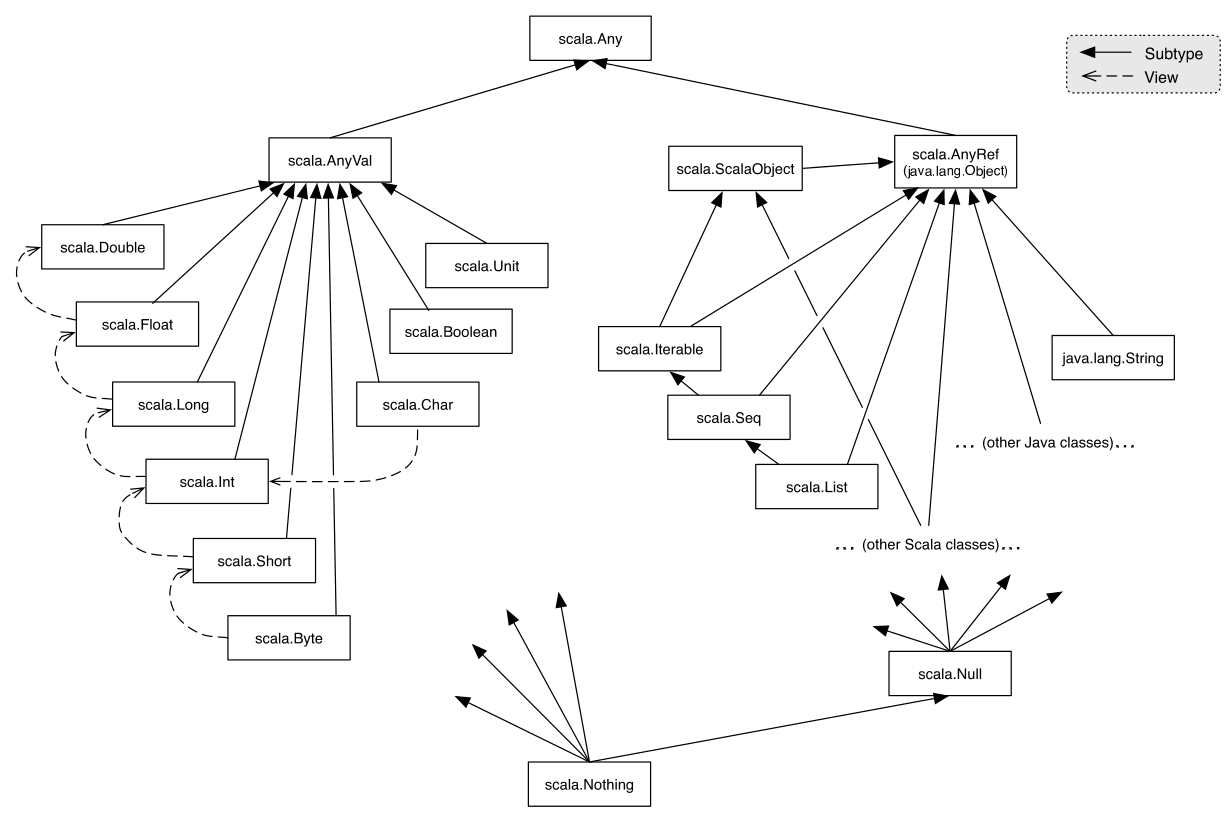
\includegraphics[width=1\textwidth]{images/scala_type_hierarchy.png}
  \caption{Scala-Commander.}
  \label{fig:scala_type_hierarchy}  
\end{figure}

Note that there are also conversions defined between primitive types, as figure \ref{fig:scala_type_hierarchy} shows using dashed arrows.

\subsubsection{Classes}

A class is declared in the following way:

\begin{lstlisting}
class C[typeParams](classParams) extends Superclass with Trait {
  definitions
}
\end{lstlisting}

With the exception of the class name, everything can be omitted. A class may extend (or \emph{mix in}) multiple traits (similarly to interfaces and abstract classes in Java). The class parameters are Scala's equivalent of Java's constructor parameters.

A class can be instantiated with the \texttt{new} operator, similar to Java.

\subsubsection{Singleton objects and companion objects}

With the use of the \texttt{object} keyword, it is possible to declare a singleton object:
\begin{lstlisting}
object O extends Superclass with Trait {
  definitions
}
\end{lstlisting}

Package-level singleton objects can define fields and methods that are accessible throughout the entire application, and thus are similar to Java's static fields and methods. In addition to that, a singleton object can have a base class or can extend traits, which is not directly possible in Java.

A \emph{companion object} is a singleton object that has the same name as a class defined in the same scope. For example:

\begin{lstlisting}
class Complex(val r: Double, val i: Double) {
  def +(c: Complex): Complex = \dots
}
object Complex {
  val zero = new Complex(0, 0)
  val one =  new Complex(1, 0)
  val i = new Complex(0, 1)
  def apply(r: Double = 0, i: Double = 0) = new Complex(r, i)
}

val c1 = Complex(2) // calls Complex.apply(2)
val c2 = Complex(2, -1) // calls Complex.apply(2, 3)
val c3 = Complex() // calls Complex.apply(0, 0)
val c4 = Complex(i = 1) // calls Complex.apply(0, 1)
val c5 = new Complex(2, 3)
val c6 = Complex.one + Complex.i
\end{lstlisting}

This is in direct parallel with a class in Java having both static and instance members: the members defined in the companion object correspond to the the static members, and the members defined in the class correspond to the intance members. Note that this is also actually how classes with companion objects are implemented in Scala (the compiler generates only one class with static and instance members).

The above example uses Scala's equivalent of overloading the method call operator \texttt{()}: the expression \texttt{a(x)} is equivalent to \texttt{a.apply(x)} where \texttt{a} is an object of a type that defines the method \texttt{apply}.

\subsubsection{Traits}

Traits are Scala's replacement for Java interfaces. In Java versions prior to 8, interfaces are highly restricted, able to contain only abstract method declarations. This leads to difficulties with convenience methods (the same methods must be reimplemented in each implementing class), and to the inability to add methods to an interface without breaking compatibility (issue for published libraries). Traits in Scala are similar to an abstract class in Java: besides defining abstract methods (just as an interface), they can provide implementations for methods, and can even have fields. A trait can extend an extend one or more other traits, and even classes. The only limitation of a trait a trait cannot have parameters (constructors).

\subsection{Syntactic flexibility}
Scala has significantly more flexible syntax when compared to Java. This includes:
\begin{itemize}

\item Semicolons are unnecessary for statements that are otherwise delimited by new lines. Semicolons are used only when more than one statement is present on a line.

\item Any method can be used as an infix operator. For example, \texttt{"\%d apples".format(count)} is equivalent to \texttt{"\% apples" format count}. This is in fact how operator overloading is possible: since method names can consist of any characters, it is possible to define a method with a symbol in its name, and then use the method as an infix operator. For example: 

\begin{lstlisting}
class Complex(val r: Double, val i: Double) {
  def +(c: Complex) = new Complex(r + c.r, i + c.i)
  def multiplyBy(c: Complex) = \dots
}
val a = new Complex(1, 2)
val b = new Complex(3, -1)
val sum1 = a + b // sum1 and sum2 are equivalent
val sum2 = a.+(b)
val prod1 = a multiplyBy b // prod1 and prod2 are equivalent
val prod2 = a.multiplyBy(b)
\end{lstlisting}

\item Possible to overload the function call operator --- methods \texttt{apply} and \texttt{update} have shorts forms similar to function calls. For example, where \texttt{a} is a class instance or singleton object, \texttt{a()} is equivalent to \texttt{a.apply()}. The method can parameters as well, e.g. \texttt{a(42)} is equivalent to \texttt{a.apply(42)}. The method \texttt{update} has an equivalent assignment-like syntax: \texttt{a() = 42} is equivalent to \texttt{a.update(42)}, and \texttt{a(4) = 2} is equivalent to \texttt{a.update(4, 2)}.

\item Scala supports the Uniform Access Principle: it is transparent to the user of a class whether a property of an object is implemented by directly using a field or by using getter-setter methods. In Scala, public \texttt{val} or \texttt{var} members can be overridden by getter-setter methods and vice-versa. This is in contrary to Java, where explicit getter-setter methods are required and the public fields exposed by a class cannot be overridden by getter-setter methods in subclasses. For example:

\begin{lstlisting}
trait Person {
  var name: String // abstract
}

class Student extends Person {
  private var _name: String
  def name = _name
  def name_=(newName: String) { _name = newName }
}

val p: Person = new Student
p.name = "Foo Bar"
println(p.name)
\end{lstlisting}

\item Scala supports the definition of constructs that are similar to language structures. For example:
\begin{lstlisting}
def safe(f: => Unit) {
  try {
    f()
  } catch {
    case e: Throwable => e.printStackTrace()
  }
}

safe {
  println("This block never throws exceptions")
}
\end{lstlisting}

In the above example, the method call parenthesis were omitted, and the block was automatically converted to an argument of type \texttt{=> Unit} which represents nullary functions returning Unit (equivalent of the Java type \texttt{void}).

\end{itemize}

This syntactic flexibility allows domain-specific languages to be defined in Scala without the need to extend the compiler. For example, the library \emph{Scala-react} defines a custom control-flow language with the use of higher-order functions, by using extensively using \texttt{apply} and \texttt{update} methods, and by using infix method call syntax for operator methods.

\subsection{Tail recursion}

Tail call optimization is an optimization technique in which method invocation instructions are replaced with jump instructions when the method invocation is immediately followed by a return from the method, effectively meaning that the method call is the last expression in the method body. The purpose if this implementation is to avoid growing the stack unnecessarily, allowing long call chains that would otherwise run out of stack space. A simple example:

\begin{lstlisting}
def a(x: Int): Int = { 
  val y = b*4
  b(y) // calling b is the returned expression 
} 
def b(x: Int): Int = { x + 2 }
\end{lstlisting} 

A special case of tail call optimization is \emph{tail recursion}, where the method being called might lead to invoking the same method again: it's either a direct call to the very same method (direct tail recursion), or a call to an other method which will eventually result in the current method being called again (mutual tail recursion). Tail recursion plays an important part of functional programming as it allows the using of recursive method calls instead of loops.

Scala only offers direct tail recursion, which is realized in compiler-time. The reason is that the JVM does not support mutual tail recursion or tail call optimization - a feat that needs runtime support.\footnote{Note that this is particular to the JVM only --- the language F\# running on top of the .NET CLR \emph{does} have tail call optimization}

\begin{figure}[h!] 
\begin{lstlisting}
def factorial(n: Int): Int = {
  @tailrec def factorialAcc(acc: Int, n: Int): Int = {
    if (n <= 1) acc
    else factorialAcc(n * acc, n - 1)
  }
  factorialAcc(1, n)
}
\end{lstlisting}
\caption{Calculating factorial using tail recursion. Notice the annotation \texttt{@tailrec}.}
\label{fig:example_scala_tailrec}
\end{figure}

The Scala compiler will automatically optimize any truly tail-recursive method. If you annotate a method that you believe is tail-recursive with the \texttt{@tailrec} annotation, then the compiler will fail to compile you if the method is actually not tail-recursive. This makes the \texttt{@tailrec} annotation a good idea, both to ensure that a method is currently optimizable and that it remains optimizable as it is modified.

Note that Scala does not consider a method to be tail-recursive if it can be overridden. Thus the method must either be private, final, on an object (as opposed to a class or trait), or inside another method to be optimized.

\subsection{Functions as types}

In Scala, functions are first-class citizens. For example, one can declare a variable that references a function:
\begin{lstlisting}
val plusOne: (Int => Int) = x => x + 1
println(plusOne(2)) // prints 3
\end{lstlisting}

In this example, the type of the variable \texttt{plusOne} is \texttt{Int => Int}, which means that it's a function taking an integer and returns an integer. The form \texttt{Int => Int} is practically a syntactic sugar for the generic type \texttt{Function1[Int, Int]}.

\subsubsection{Partial functions}

A partial function in Scala is a function that is only defined for a subset of its input set. For example:
\begin{lstlisting}
val fibo: PartialFunction[Int, String] = {
  case 1 => "one"
  case 2 => "two"
  case 3 => "three"
  case 5 => "five"
  case 8 => "eight"
}

println(fibo.isDefinedAt(2) + " " + fibo(2)) // prints: true two
println(fibo.isDefinedAt(4)) // prints "false"

// prints "one two three five eight"
(0 to 10).collect(fibo).foreach(x => print(x + " "))
\end{lstlisting}

The function \texttt{fibonacci} is a partial function taking an \texttt{Int} value and returning \texttt{String}, as is defined only for the first five Fibonacci values. A partial function has two important methods: 
\begin{itemize}
\item \texttt{isDefinedAt(x)}: returns true if the partial function is defined for \texttt{x}, and returns false otherwise;
\item \texttt{apply(x)}: return the value of the function for the given \texttt{x} if the function is defined for \texttt{x}, and throws an exception otherwise.
\end{itemize}

Partial functions in Scala are used for pattern matching, or as a programmable \emph{switch-case}-like structure. For example, the event handling mechanism of \emph{Scala-Swing} uses partial functions (see section \ref{sec:theory_scala-swing-event-handling}).

\subsection{Currying}

Currying is the technique of transforming a function that takes multiple arguments (or a tuple of arguments) in such a way that it can be called as a chain of functions, each with a single argument (partial application).

Consider the following function:
\begin{lstlisting}
def sum(a: Int)(b: Int): Int = { a + b }
\end{lstlisting}
This is a curried function, which takes an integer \texttt{a} and returns a function that takes an integer \texttt{b} and returns the value \texttt{a + b}. This is just syntactic sugar for the form:
\begin{lstlisting}
def sum(a: Int): (Int => Int) = b => a + b
\end{lstlisting}
Both forms can be used in the same way:
\begin{lstlisting}
println(sum(1)(2)) // prints 3

val plusOne: (Int => Int) = sum(1)
println(plusOne(2)) // prints 3
\end{lstlisting}

Typical use cases of currying in Scala include helping type inference, providing fluent API, and performance improvements in multi-stage computation.

\subsubsection{For type inference}

In Scala, type inference of expressions on a single line always works form left to right: the leftmost expression is evaluated first, then followed by the next expression to the right. Chained function applications of curried functions are considered separate expression, and therefore type inference on a proceeding parameter can affect the type inference of a latter parameter. Consider the library function \texttt{foldLeft} defined on sequences of base type \texttt{A}:
\begin{lstlisting}
def foldLeft[B](z: B)(op: (B, A) => B): B
\end{lstlisting}
This allows the following code:
\begin{lstlisting}
val s = List("Joe", "Jack").foldLeft(0)((len, name) => len + name.length)
println(s) // prints 7
\end{lstlisting}
If \texttt{foldLeft} was defined as a simple non-curried function such as the following:
\begin{lstlisting}
def foldLeft[B](z: B, op: (B, A) => B): B
\end{lstlisting}
The one would have to provide more explicit types:
\begin{lstlisting}
List("Joe", "Jack").foldLeft(0, (len: Int, name: String) => len + name.length)
List("Joe", "Jack").foldLeft[Int](0, (len, name) => len + name.length)
\end{lstlisting}

\subsubsection{For fluent API}
Currying (together with other language features) allows to create an API that looks like a language construct:
\begin{lstlisting}
def loop[A](n: Int)(body: => A): Unit = (0 until n) foreach (n => body)

loop(2) {
   println("hello!")
}
\end{lstlisting}

\subsubsection{Multi-stage computation}

Consider a problem where we want to decide whether given point is inside a given circle, identified by its center point and radius:

\begin{lstlisting}
class Point(val x: Double, val y: Double)
class Circle(val center: Point, val radius: Double)

def isInside(c: Circle, p: Point): Boolean = {
  import Math.pow
  val radiusSquare = pow(c.radius, 2)
  val distSquare = pow(p.x - c.center.x, 2) + pow(p.y - c.center.y, 2)
  distSquare <= radiusSquare
}

val myCircle = new Circle(new Point(1, 2), 2)
val points = Seq(new Point(2, 3), new Point(4, 2), new Point(1, 1))
val inside = points.map(p => isInside(myCircle, p))
println(inside) // List(true, false, true)
\end{lstlisting}

In the above example when we calculate whether a \emph{series} of points are inside the \emph{same} circle, we are calculating the value \texttt{radiusSquare} over and over again for each point, even though calculating it only once and then using it for all the points would suffice. Currying offers a simple and elegant solution:
\begin{lstlisting}
def isInside(c: Circle): (Point => Boolean) = {
  import Math.pow
  val radiusSquare = pow(c.radius, 2)

  (p: Point) => {
    val distSquare = pow(p.x - c.center.x, 2) + pow(p.y - c.center.y, 2)
    radiusSquare >= distSquare
  }
}

val myCircle = new Circle(new Point(1, 2), 2)
val points = Seq(new Point(2, 3), new Point(4, 2), new Point(1, 1))
val isInsideMyCircle = isInside(myCircle)
val inside = points.map(p => isInsideMyCircle(p))
println(inside) // List(true, false, true)
\end{lstlisting}

Now the function \texttt{isInsideMyCircle} already has the value \texttt{radiusSquare} pre-calculated. Note that in this case using the simple multi-parameter list version of currying does not offer the same performance benefits, because Scala cannot automatically transform the function body to extract computation that is dependent only on a subset of the parameters.

\subsubsection{Partially applied functions}

Partial function application and currying are related. One of the significant differences between the two is that a call to a partially applied function returns the result right away, not another function down the currying chain; this distinction can be illustrated clearly for functions whose arity is greater than two.

Let us consider the following example:
\begin{lstlisting}
def sum3(a: Int, b: Int, c: Int) = a + b + c
val sum2: ((Int, Int) => Int) = sum3(1, _: Int, _: Int)
println(sum2(2, 3)) // prints 6
\end{lstlisting}

After fixing the first parameter to the value \texttt{1}, the function \texttt{sum2} is a binary function, taking two arguments. This is in contrast to what it would be if \texttt{sum3} were a curried function:
\begin{lstlisting}
def sum3(a: Int)(b: Int)(c: Int) = a + b + c
val sum2: (Int => Int => Int) = sum3(1)
println(sum2(2)(3)) // prints 6
\end{lstlisting}

\section{Scala-swing}\label{sec:theory_scala-swing}

Scala-swing is a UI library written in Scala that wraps the Java Swing components with the purpose of providing a simpler, more straightforward and typesafe interface that is more natural to use in Scala. It is meant to be sufficiently close to the Java Swing to appeal to Java programmers with existing Swing experience.\cite{ScalaSwing} The library diverges significantly from Java Swing only on parts that are considered as bad design decisions of Java Swing.

The library provides lightweight wrappers around Swing components, maintaining their functionality and hierarchy, reimplementing them in Scala-like terms (using Scala properties instead of getter/setter methods, using enumerations instead of magic constants, and providing a typesafe API for objects like JList). The main divergences are the following:
\begin{itemize}
\item In Java Swing all components are also containers. This doesn't make sense for a number of components (e.g. TextField, CheckBox, Button etc.) This is likely to be because of the lack of multiple inheritance in Java. Scala-swing uses the \emph{trait} \texttt{Container}.

\item Layout managers and panels are coupled, though they are decoupled in Java Swing. Scala-swing offers a straightforward, typesafe API for the standard Swing layout managers in the form of a panel class for each layout (e.g. \texttt{BorderPanel} for a \texttt{JPanel} with \texttt{BorderLayout}).

\item The event mechanism is completely reworked around the concept of publishers and reactors. This offers a more homogeneous API for event management than what Java Swing offers.
\end{itemize}

\subsection{Event handling}\label{sec:theory_scala-swing-event-handling}

Event handling is based around the concepts of \emph{publishers} and \emph{reactors}. Any \texttt{scala.\-swing} component is actually both a publisher that publishes events and a reactor that reacts to events. For efficiency reasons, events of a component are not published directly by the component itself but by members, grouping the events into categories (see below the member \texttt{mouse}).

As each event is a normal Scala object, it has a unique type, which determines how to pattern match on it. Contrast this to Java Swing, where some events are dispatched in two phases, according to their type plus an additional listener method. The following example shows how to listen to mouse click events using Java Swing:
\begin{lstlisting}
new JComponent {
  addMouseListener(new MouseAdapter {
    @Override
    def mouseClicked(e: MouseEvent) {
      System.out.println("Mouse clicked at " + e.getPoint)
    }
  })
}
\end{lstlisting}

Note that in this case we are using the convenience class \texttt{Mouse\-Adapter} that implements all the methods of the interface \texttt{Mouse\-Listener} with empty implementations. This interface is just one example where we first dispatch by the event's Java type (\texttt{MouseEvent}) and then we refine the match implementing the appropriate method (\texttt{mouseClicked}). The equivalent using \texttt{scala.swing} looks like the following:
\begin{lstlisting}
new Component {
  listenTo(mouse.clicks)
  reactions += {
    case e: MouseClicked =>
      println("Mouse clicked at " + e.point)
  }
}
\end{lstlisting}

Here we rely on the event type (\texttt{MouseClicked}). Since the event classes form hierarchies, we can also very conveniently listen to \emph{any} mouse event:
\begin{lstlisting}
  listenTo(mouse.clicks, mouse.moves, mouse.wheel)
  reactions += {
    case e: MouseEvent =>
      println("Mouse event at point " + e.point)
  }
\end{lstlisting}

The equivalent using Java Swing would require us to add three listeners (using \texttt{add\-Mouse\-Listener}, \texttt{add\-Mouse\-Motion\-Listener}, \texttt{add\-Mouse\-Wheel\-Listener}) and to implement a total number of \textbf{eight listener methods}, all with the same implementation.

Note that the members \texttt{listenTo} and \texttt{reactions} are defined by the trait \texttt{Reactor}. The member \texttt{reactions} is a mutable list of \emph{partial functions} of type type \texttt{PartialFunction[Event, Unit]}.

\section{Scala CPS Plugin}\label{sec:theory_scala-cps-plugin}

Delimited continuations are a versatile programming tool. Their most important use is based on their ability to suspend and resume sequential code paths in a controlled way. The Scala CPS plugin is a compiler plugin that enables the programmer to have delimited continuations in direct-style code, without much syntactic overhead. This is implemented by the plugin selectively transforming the source code in compile time, driven by annotations and other structures placed into the code by the programmer. Multiple variants of delimited continuations have been described in the literature, and the Scala CPS plugin implements the so-called Danvy and Filinski model, with two primitive operations, \texttt{shift} and \texttt{reset}.

A delimited continuation embodies a certain part of the program. When invoking a delimited continuation, the control returned to the caller, and it may also return a value. Inside the continuation, at any point the current fragment of the call stack starting from the delimiting block can be saved to be later reused (possibly multiple times), or discarded. This control over the execution of the control flow can is the essence of the delimited continuations.

Since the Scala CPS plugin uses compile-time transformation, applications using it do not need a special VM or other specific runtime support.

\subsection{\texttt{shift} and \texttt{reset}}

There are two control operators: \texttt{shift} and \texttt{reset}. The \texttt{reset} operator is followed by a code block which is the continuation itself. The \texttt{shift} blocks inside the continuation play a dual role: 
\begin{itemize}
\item they are in control of the rest of the continuation: the rest of the continuation is provided in the form of a function (denoted as \texttt{k} below), and the \texttt{shift} block can decide what to do with it: it may invoke it once, more than once, or never. Note that the rest of the continuation may include further \texttt{shift} blocks;
\item the value returned in the \texttt{shift} block gets propagated back to the previous \texttt{shift} block (as the result of the function \texttt{k}), or, in case of the first \texttt{shift} block, back to the \texttt{reset} block itself.
\end{itemize}

The value of the \texttt{reset} block is always equal to the return result of the very first \texttt{shift} block that gets executed in the continuation, or, in case no \texttt{shift} block gets executed, equal to the body of the \texttt{reset} block (see figure  \ref{fig:example_cps_no_shift}).

\begin{figure}[h!] 
\begin{lstlisting}
val simple: Int = reset {
  val a = 40
  val b = 2
  a + b
}
println(simple) // 42
\end{lstlisting}
\caption{No \texttt{shift} block - the continuation is executed sequentially.}
\label{fig:example_cps_no_shift}
\end{figure}

Figure \ref{fig:example_cps_generic} shows a simple \texttt{reset} block with a single \texttt{shift} block inside and also shows an equivalent manually transformed version of the same continuation. In this example, the shift block invokes the rest of the continuation, which in the \(x+4\) function, with the argument 1, modifies the result by adding 7 to it, and returns the result (12). Because this is the only \texttt{shift} block in the continuation, the returned value is the result of the \texttt{reset} block.

\begin{figure}[h!]
 
\begin{tabular}{ C{7cm}  C{8cm}}

\begin{lstlisting}
val result = reset {
  val s = shift {
    k: (Int => Int) =>
      k(1) + 7
  }
  s + 4
}
println(result) // prints 12
\end{lstlisting}
&
\begin{lstlisting}
val reset = {
  val shift: ((Int => Int) => Int) = {
    k: (Int => Int) =>
      k(1) + 7
  }
  val rest: (Int => Int) = {
    s: Int =>
      s + 4
  }
  shift(rest)
}
println(reset) // prints 12
\end{lstlisting}
\\
\end{tabular}
\caption{Left is a delimited continuation, and right is the equivalent manually-transformed CPS versions.}
\label{fig:example_cps_generic}
\end{figure}

\subsubsection{Answer type modification}

The Scala CPS plugin allows full answer type polymorphism in a statically type-safe manner. This allows the return type of the \texttt{reset} block (the type of the last expression in the block) and the return type of the individual \texttt{shift} blocks to be different. The transformation accurately tracks answer-type modification throughout the continuation and ensures, in compile time, that no type errors can occur in runtime (u.i. if the continuation can possibly run through path of conflicting answer types, the compilation fails with error.)

Figure \ref{fig:example_cps_answer_type_modification} shows a simple an example where answer-type modification takes place. The type of the entire continuation is \texttt{String}, the answer type of the \texttt{reset} block is \texttt{Int}, and the answer type is modified in the \texttt{shift} block from \texttt{Int} to \texttt{String}. Note that even though the \texttt{shift} block's body returns a \texttt{String} (which the final answer type of the continuation), the actual type of the \texttt{shift} \emph{expression} is a third type \texttt{Char}, which corresponds to the input type of the function \texttt{k}.

\begin{figure}[h!] 
\begin{lstlisting}
def charToHexString(char: Char): String = {
  reset {
    val c: Char = shift {
      k: (Char => Int) =>
        val num: Int = k(char)
        "0x%02x".format(num) // Int to String (hex code)
    }
    c.toInt // converts Char to Int
  }
}
println(charToHexString('A'))
\end{lstlisting}
\caption{An example showing answer type modification: the continuation's type is \texttt{String} even though the \texttt{reset} block's body returns \texttt{Int}.}
\label{fig:example_cps_answer_type_modification}
\end{figure}

\subsubsection{Dynamic control flow}

A delimited continuation does not has to consist of a single block that the compiler can understand entirely. It is possible to have \texttt{shift} blocks defined in methods or functions, and thus the \texttt{shift} blocks to be associated only in runtime with a certain \texttt{reset} block. Since the final return type of the \texttt{reset} block is not necessarily reflected in a \texttt{shift} block at all (because of answer type polymorphism), the code containing such ``detached'' \texttt{shift} blocks \textbf{must} be annotated with the annotation \texttt{@cpsParam[B, C]} where \texttt{B} is the type of computation state after computation has executed, and before control is returned to the shift, and \texttt{C} is the eventual return type of this delimited computation. 

Because the compiler needs to transform CPS code, non-CPS code cannot (neither directly nor indirectly) call CPS-code. This can lead to awkward limitations, such as the inability to iterate through a sequence with a simple for-loop (the reason is that a for-loop is desugareted by the compiler to a \texttt{foreach} method call on the collection with the loop as a closure body being the argument). Code that needs to interact with CPS-code thus needs to be marked to CPS-code itself (by the annotation @cpsParam), but then such code can no longer be used by non-CPS code (even if it doesn't contain \texttt{shift} blocks). A reason is that a method returning the type \texttt{A} annotated with \texttt{@cpsParam[B,C]} is effectively transformed by the compiler to return the internal type \texttt{ControlContext[A,B,C]}. 

\fullref{chap:cps-examples} contains examples demonstrating the annotation @cpsParam.

\subsection{Use cases}

The paper \cite{CPSTransform} describes some academic use cases (Type-Safe printf, Direct-Style Monads, Concurrency Primitives, Actors, Functional Reactive Programming, Asynchronous IO). At the time of writing, the following widely available Scala libraries using delimited continuations were available:
\begin{itemize}
\item Akka Dataflow Concurrency --- Akka implements Oz-style dataflow concurrency by using a special API for \emph{Futures} that enables a complementary way of writing synchronous-looking code that in reality is asynchronous. \cite{AkkaDataflow}
\item Scala.React --- A reactive programming library for Scala developed based on the paper \cite{DeprecatingObservers}.

\end{itemize}

%There are typically two use cases of delimited continuations. In cases where the \texttt{reset} block returns a value, the continuation itself is typically runs to its end, with the return results being the primary meaning of the computation which is directly returned to the invoker of the \texttt{reset} block. This is similar to how an ordinary computation (without delimited continuations) would obtain its value.

%In cases where the return type of the continuation is of type \texttt{Unit}, the continuation is only invoked for its \emph{side effect}. In this case, the state of the continuation is typically \emph{stored} somewhere in the system to be later executed, and the invoker of the \texttt{reset} block typically gets the control back before the rest of the continuation would be executed. In this case, the answer type is \texttt{Unit}, and the annotation \texttt{@cpsParam[Unit, Unit]} has its own alias in the form \texttt{@suspendable}.



\section{Scala.React}\label{sec:theory_scala-react}

Programming systems with interactive user interfaces requires a considerable amount of engineering to deal with continuous user input and output, yet the predominant programming models dealing with continuous state change in applications is the observer pattern. The Scala library \emph{Scala.React} offers a reactive data-flow programming model, and by that it solves numerous engineering problems observer pattern-based design faces. Amongst multiple Scala features, this is enabled by the higher order concepts of events and state, enabled by Scala's higher-order functions, and by a data-flow DSL embedded into Scala, enabled by continuation passing style transformation that \emph{Scala} offers. Its design is also heavily based on Scala's \emph{traits}, simplifying the binding of observer-based interfaces to the reactive abstractions.\cite{DeprecatingObservers}

TODO: detailed list of benefits of using scala.react when compared to traditional observer pattern - each should be explained below

\subsection{Event streams}

The base of simplifying the event logic is a general interface, offering uniformity, abstraction and reusability. The class {\tt EventSource[A]} represents a generic source of events of type {\tt A}. It is possible to schedule an event source to emit a value at any time. Let us consider an example of an event source of type integer emitting two events:
\begin{lstlisting}
val es = new EventSource[Int]
es emit 1; es emit 2
\end{lstlisting}

We can print all events from the event source to the console as follows:
\begin{lstlisting}
val ob = observe(es) { x => println("Receiving " + x) }
\end{lstlisting}

In case of a UI application, we can have a button class that emits event each time the button is pressed. The values associated with the event might represent the click count:

\begin{lstlisting}
class Button(label: String) {
  val clicks = new EventSource[Int]
  // for each event coming from the UI component, call "clicks emit x"
}
\end{lstlisting}

It is possible to listen to an event, and associate an action that needs to be executed when the event emits. In a UI application, we can have a ``Quit'' button that terminates the application.
\begin{lstlisting}
val quitButton = new Button("Quit")
observe(quitButton.clicks) { _ => System.exit() }
\end{lstlisting}

\subsection{Signals}

Many interactive application needs to deal with continuously changing values. Usually, changes made to internal variables needs to be reflected on the UI, possibly in more than one place. We can represent time-varying values by the type \texttt{Signal}. A signal is an observable object that has an associated value in any point of time. There are two main kind of signals: variables and functions (either strictly or lazily evaluated, see below).

Let us consider a fragment of a file manager application that displays, in the form of a label, a text with the number of selected files and folders.

\begin{lstlisting}
val selectedFiles: Var[Int]
val selectedFolders: Var[Int]
val selection: Strict[String] { "There are " + selectedFiles() + " files(s) and " + selectedFolders() + " folder(s) selected".

observe(selection) {
  selectionStr => selectionLabel.text = selectionStr
}
\end{lstlisting}

In the above example, whenever the number of selected files and folders changes, the signal \texttt{selection} is automatically evaluated, and the component on the UI is automatically updated. 

In this example, the signal is \texttt{Strict}, which means that whenever the dependent signals (\texttt{selectedFiles} and \texttt{selectedFolders}) change their value, the signal is automatically re-evaluated. We need this because we always want to keep the UI updated. For cases where this is not necessary, we can use the type \texttt{Lazy} that represents a signal function that is evaluated only if needed. This means that an observer listening to such lazy signals might miss events.

\subsection{Reactives}

Events and signals are very tightly related concepts. They are both \emph{reactives}. The widely used method \texttt{observe} expects a reactive, therefore it possible to observe an event source or a signal the same way. The difference between them is only subtle: while a signal always has a defined value, and event source only has a value while it is \emph{emitting} (it does not store the value emitted last time). There are also operations that lets convert between the two: the trait \texttt{Signal[A]} defines the method \texttt{changes} that creates an event source for the current signal; and the trait \texttt{Events[A]} defines the method \texttt{hold} that creates a signal that always holds the values of current event (and has a given initial value).

\subsection{Reactors: observers without inversion of control}

One of the most important issues with having to deal with observer-based architecture is the \emph{inversion of control}. When an operation consisting of multiple events needs to be modeled, the typical solution is to model it as a \emph{state machine}. 

Let us consider a simple drawing application that lets us draw a closed line using the mouse (variables \texttt{mouseDown}, \texttt{mouseMove} and \texttt{mouseUp} are event sources):

\begin{lstlisting}
var moveObserver: Observer = null
var path: Path = null
observe(mouseDown) {
  downPos => 
    path = new Path(downPos) // new path with a starting position
    moveObserver = observe(mouseMove) {
      movePos =>
        path.add(movePos) // add the current position to the path
        draw(path)
    }
}

observe(mouseUp) {
  _ =>
    moveObserver.dispose()
    path.close() // closes the path
    draw(path)
}
\end{lstlisting}

The above example has multiple fundamental issues. The drawing logic is inverted (scattered through three observer blocks), the observers needs to be manually disposed, and it is prone to errors (e.g. if a mouse up event is somehow triggered without a mouse down event, the code fails with a null-pointer runtime exceptions --- a defensive code would increase complexity).

Ideally, we want to encode a state-machine that can be described informally as follows:
\begin{enumerate}
\item Once the mouse button is pressed, start a new path.
\item While the mouse isn't released, gather all mouse moves and draw the path.
\item Once the mouse is released, close and draw the path.
\end{enumerate}

Scala.React's imperative data-flow language and the concept of \emph{reactors} lets us turn the above steps into a straightforward implementation:

\begin{lstlisting}
Reactor.loop { self =>
  val initialPos = self await mouseDown
  val path = new Path(initialPos)
  self.loopUntil(mouseUp) {
    val movePos = self awaitNext mouseMove
    path.add(movePos)
    draw(path)
  }
  path.close()
  draw(path)
}
\end{lstlisting}

The method \texttt{Reactor.loop} creates a reactor that repeatedly executes the given block. The variable \texttt{self} lets us control the reactor, which supports actions such as \texttt{await}, \texttt{awaitNext} and \texttt{loopUntil}. The actions \texttt{await} and \texttt{awaitNext} pauses the reactor until the given event source emits; whenever it does emit, the reactor is resumed from exactly where it was paused, with all its internal state (e.g. \texttt{path}) restored. This is enabled by the Scala CPS plugin: the method \texttt{loop} contains a \texttt{reset} block, and the methods \texttt{await} and \texttt{awaitNext} contain a corresponding \texttt{shift} block that creates an observer on the given event source that resumes the continuation. For more details, see \ref{sec:scala-react-impl}.

\subsection{Data-flow language}

Scala-React's data-flow language has a series of operations on reactors that offers control over the reactor:
\begin{itemize}
\item \texttt{flow}: creates a new reactor with a control flow that is executed once;
\item \texttt{loop}: creates a new reactor with a control flow that is repeatedly executed, until the reactor is disposed or the reactor calls the \texttt{join} method on itself;
\item \texttt{await}: waits for the given reactive to emit; if it is already emitting in the current cycle, this method immediately returns;
\item \texttt{awaitNext}: waits for the given reactive to emit; if it is already emitting, it discards the current value and awaits for the next;
\item \texttt{pause}: suspends the reactor which will be continued in the next iteration --- useful to break infinite cycles in reactors or to run a have a long-running operation on the UI without completely blocking (freezing) it;
\item \texttt{halt}: suspends and disposes the reactor;
\item \texttt{par}: lets execute \emph{two} branches in \emph{parallel}, until they both finish or until or at least one calls the method \texttt{join}; useful in cases we want to have two related control flows that in control of each other;
\item \texttt{join}: halts the reactor or controls the enclosing \texttt{par} expression;
\item \texttt{abortOn}: discards a reactor block as soon as a given reactive emits; useful if we need a control flow that supports \emph{cancelling} of whatever action it is doing;
\end{itemize}

\subsection{Implementation details}\label{sec:scala-react-impl}

Scala.React proceeds in discreet steps, called \emph{turns}. Part of the implementation is a \emph{scheduler} and a \emph{propagator}. External updates, such as when an event source is triggered, are forwarded to the scheduler which schedules a revalidation request for the next turn. In the next turn, the propagator takes over, and revalidates all related events and signals, possibly creating other turns (e.g. when there is a dependent signal on a signal being updated). This turn-by-turn evaluation strategy makes it possible that the system is always in a consistent state (e.g. it's \emph{glitch-free}). 

\subsubsection{Signal expressions}

Scala.React propagates changes and resolves dependencies using an internal representation of \emph{nodes} forming a \emph{tree}. Event sources and signals are represented as such nodes. As part of the revalidation, subtrees are inspected and, in case of opaque nodes (see below), are rebuilt.

A signal can depend on other signals; whenever the \emph{dependent} signals change their value, the \emph{depending} signal needs to be notified (e.g. to be re-evaluated in case of strict signals). This means that there is an implicit observer-subject relationship between such signals. Maintaining such relationship is straightforward for derived signals such as \texttt{val s1 = s0.map(\dots)} where it is statically known that \texttt{s1} depends on \texttt{s0}. A signal expression of the form \texttt{Strict\{ a() + b()\}} however is completely opaque to the framework (the block is a closure), e.g. it has no prior knowledge that it depends on the signals \texttt{a} and \texttt{b} before actually evaluating it. The nodes of such signals are therefore called \emph{opaque} nodes.

When defining a signal such as \texttt{Strict\{ a() + b()\}} we are in fact calling a factory method 
\begin{lstlisting}
def Signal[A](op: =>A): Signal[A]
\end{lstlisting}
with the argument \texttt{\{ a() + b()\}}. The compiler rewrites the expressions \texttt{a()} and \texttt{b()} to method calls \texttt{a.apply()} and \texttt{b.apply()}, which are important below. The parameter \texttt{op} of the factory method \texttt{Signal} with the type \texttt{=> A} is actually a ``call-by-name'' argument (a nullary function). This means that the expression in the closure body does not get evaluated when the signal is created, but instead it is passed to the newly created signal object. The actual body of the signal is evaluated during a revalidation turn, which uses an internal stack for establish dependencies: before evaluating the above signal expression, the signal is pushed to the stack; during the evaluation of the signal expression if the execution gets to an \texttt{apply} method of a signal, the topmost element on the stack is added to the dependents list of the signal. This way, dependencies are automatically discovered, without the need of explicitly stating them.

For some language expressions, dependencies can actually vary. Consider the signal
\begin{lstlisting}
val s = Signal { if (c()) a() else b() }
\end{lstlisting}
Signal \texttt{s} should ideally ever depend on only two signal: on signal \texttt{c} and either \texttt{a} or \texttt{b} (depending on \texttt{c}'s value). Therefore, when a node notifies its dependencies of a change, it removes all opaque dependents (and expects them to re-add themselves as needed).


\subsubsection{Lifecycle management of observers}






\section{FEST-Swing}\label{sec:theory_fest-swing}

FEST (Fixtures for Easy Software Testing) is a collection of libraries whose mission is to simplify software testing. It is composed of various modules, which can be used with TestNG or JUnit. The most significant module is the FEST-Swing module.

The Swing module provides a simple and intuitive API for functional testing of Swing user interfaces, resulting in tests that are compact, easy to write, and read like a specification. Tests written using FEST-Swing are also robust. FEST simulates actual user gestures at the operating system level, ensuring that the application will behave correctly in front of the user. It also provides a reliable mechanism for GUI component lookup that ensures that changes in the GUI's layout or look-and-feel will not break the tests \cite{FESTMain}.

\subsection{Introduction}

A FEST-Swing test is testing either individual frames (the building blocks of a UI), or entire Swing applications or Applets. FEST simulates actual user gestures (mouse movements, keys presses) at the operating system level, ensuring that during the application will behave in the same way as in the front of the user. It uses AWT Robot, which generates events in the platform's native input queue. Thus, the test needs to create the components and make them visible on the screen, and the tests will actually moves the mouse cursor, and not just only generates mouse move events.

\subsection{Architecture}

FEST Swing's component fixture architecture is separated into several layers (from bottom to top):
\begin{enumerate}
\item BasicRobot: Simulates a user interacting with a mouse and keyboard. It uses the AWT Robot to generate native input events.
\item Component driver: This layer does all the ``heavy lifting.'' All interaction with a GUI component is done in this layer. It knows how to simulate events and check the state of a specific GUI component. For example, JComboBoxDriver knows how to simulate a user using a JComboBox (selecting a particular element) and how to verify the state of it (which element should be selected.)
\item Component fixture: This layer sits on top of the driver. It provides a fluent interface to that and makes the API easier to write and read. Users of FEST write their GUI tests using fixtures, not drivers. There is one fixture per Swing component, and each fixture has the same name as the Swing component they can handle ending with ``Fixture.'' For example, a JButtonFixture knows how to simulate user interaction and verify state of a JButton. Fixtures can be considered the ``user interface'' of the FEST-Swing library.
\end{enumerate}

The architecture also supports extensions, so developers of application using custom Swing components can write their own fixtures and component drivers.

\subsection{Example}

Writers of GUI tests need to use the fixtures located in the package org.fest.swing.fixture. These fixtures provide specific methods to simulate user interaction with a GUI component and they provide assertion methods that verify the state of the GUI component. Although it is possible to work with the FEST BasicRobot directly, the BasicRobot is too low-level and requires considerably more code than the fixtures.

As a concrete example, let us consider a very simple JFrame that contains a JTextField, a JLabel and a JButton, and component has its unique name. The expected behavior of this GUI is the following: when user clicks on the JButton, the text of the JTextField should be copied to the JLabel. (Figure \ref{fig:example_jframe}) 

\begin{figure}[h!] \label{fig:example_jframe}  
  \centering
    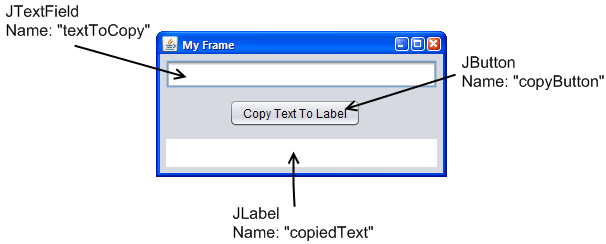
\includegraphics[width=0.6\textwidth]{images/example_jframe.png}
  \caption{A very simple JFrame that contains a JTextField, a JLabel and a JButton.}
\end{figure}

To the frame, the test's setup method needs to create the frame (in the EDT, delegating it with GuiActionRunner), create a fixture for it, and make it visible (Figure \ref{fig:example_setup_method}).

\begin{figure}[h!] \label{fig:example_setup_method}
\begin{lstlisting}
protected def onSetUp() : Unit = {
    val frame : MyFrame = GuiActionRunner.execute(new GuiQuery[MyFrame] {
        protected def executeInEDT() : MyFrame = new MyFrame
    })
    window = new FrameFixture(robot, frame)
    window.show() // shows the frame to test
}
\end{lstlisting}
\caption{The setup method creating the frame and the fixture, and making it visible.}
\end{figure}

The test method can use the fixture to simulate a user interacting with a GUI in order to verify that such GUI behaves as we expect. The user interactions and the assertions in the test are fluent and simple. The method looks up the UI components by their unique names. (Figure \ref{fig:example_test_method})

\begin{figure}[h!] \label{fig:example_test_method}
\begin{lstlisting}
@Test 
def shouldCopyTextInLabelWhenClickingButton : Unit = {
    window.textBox("textToCopy").enterText("Some random text")
    window.button("copyButton").click()
    window.label("copiedText").requireText("Some random text")
}
\end{lstlisting}
\caption{The test method.}
\end{figure}

It is important to mention that besides testing individual components that build up an application, FEST-Swing also supports testing entire applications. In such cases, the first tests starts up the application with ApplicationLauncher that understands how to launch an application using its main method. Once the application is started, the test just needs to find the application's main window.

\subsection{Threading model}

The documentation of FEST-Swing strongly advises to respect Swing's threading rules \cite{OracleSwingThreading} both in the tests and in the tested application (this remains only an advice because Swing itself does not enforce thread safety). In short, the cardinal rule is the following: creation and access (both read and write) of Swing components should be done in the Event Dispatch Thread (EDT.) Since JUnit and TestNG tests do not run on the EDT, creation and any direct access in the tests to Swing components should be delegated to EDT via the utility class GuiActionRunner (or via other tools).

To ensure that the threading rules are respected throughout the tests and the tested application, FEST Swing provides the class FailOnThreadViolationRepaintManager. It forces a test failure if access to Swing components is not performed on the EDT. However, it only detects component creation and writing, and is unable to detect read operations (component creation and writing triggers repaint events, but read does not).

\subsection{Limitations}\label{sec:fest-swing-limitations}

Because FEST-Swing is actually simulating user interaction, it needs an environment very similar to actual user environments: the tested application needs to be active and in focus, and needs to move the mouse. Therefore, that machine that the tests run on cannot be used for the entire duration of the tests. In addition, the tests probably fail whenever another applications unexpectedly gets the focus and covers the application's window (the mouse no longer clicks the correct application). This can become a burden because UI tests, by their nature, can take a significant amount of time to execute and especially when using agile development methods, it is preferable to run them frequently.

Because of this, it is common to delegate the tests to Continuous Integration (CI) systems (e.g. Hudson/Jenkins, TeamCity etc.) When the CI platform is based Linux, BSD or UNIX-style operating systems, it is common that the server does not even have the X Window system, running applications with UI impossible. For this case, Xvfb offers a simple and straightforward solution \cite{FESTxvfb}.

However, if the target platform is Windows, there are a whole set of issues, and the known solutions are problematic, and are very complicated and time consuming to setup. \cite{HudsonUnderWindows} \cite{Cacio_Tta_FEST}

To overcome all of these limitations, OpenJDK's project Caciocavallo can be used \cite{Cacio_Tta_FEST} to provide a graphics stack for the Java VM that is completely independent from the environment, eliminating any need for platform-dependent setup for CI systems. It renders everything into a virtual screen (which is simply a BufferedImage object), and is driven solely by AWT Robot events. However, this also has its own limitations; the most important being that drag-and-drop \cite{IntroDnD} is unsupported, thus it needs certain workarounds (see \fullref{sec:simulated-dnd}).

\section{Design patterns}\label{sec:theory_design-patterns}

\subsection{Model-View-Controller}\label{sec:model-view-controller}

Model-View-Controller is an architectural pattern for implementing user interfaces. It divides an application into three connected parts:
\begin{itemize}
\item \textbf{Model} --- consists of the application data, business rules, logic and functions;
\item \textbf{View} --- consists of the visual representation of the data, along with components that a user can interact with (e.g. consists of the Java Swing components);
\item \textbf{Controller} --- accepts inputs from the view, and converts it to commands for the model or view.
\end{itemize}

The interaction between the three components is defined as follows:
\begin{itemize}
\item A \textbf{controller} knows the view and the model, it listens to events of the view triggered by the user and updates the view and the model accordingly.
\item A \textbf{view} accepts user interaction, and notifies its observers (u.i. the controller). It also listens to the changes of the model, and updates its state accordingly.
\item A \textbf{model} notifies its observers (u.i. the view) whenever its state changes.
\end{itemize}

Figure \ref{fig:mvc_pattern} shows the relation between the three components of the MVC pattern. The pattern relies on the \emph{Observer} pattern: the view is the subject of the observing controller, and the model is the subject of the observing view (hence the indirect dependencies on figure \ref{fig:mvc_pattern}).

The purpose of this separation is that the parts can be interchangeable (e.g. more than one view can exist for the same model, or more than behavior can be defined using different controllers), and are testable separately (e.g. it is possible to the test just the model without a UI, to test just the view with a mocked model, or to test the controller with mocked view and model).

\begin{figure}[h!]
\centering
\begin{tikzpicture} 
\umlemptyclass[x=0, y=0]{Model} 
\umlemptyclass[x=6, y=0]{Controller} 
\umlemptyclass[x=3, y=-2]{View} 
\umluniassoc[geometry=--]{Controller}{Model} 
\umluniassoc[geometry=--]{Controller}{View} 
\umluniassoc[geometry=--]{View}{Model} 
\umlVHdep{Model}{View}
\umlHVdep{View}{Controller}
\end{tikzpicture}
\caption{The Model-View-Controller pattern.}
\label{fig:mvc_pattern}
\end{figure}

\section{Functional testing of an application with a user interface}\label{sec:theory_functional-ui-testing}

\subsection{User Action and Adapter design pattern}\label{sec:user-actions-adapters}

The users using an application with a UI typically interact with it by executing a series of operations that change the application's state. These operations might themselves be consisting of multiple operations of the UI components, changing the UI's state and, indirectly, changing the application's internal state. UI test simulating the users can incorporate in their architecture the concept of separation: the tests can interact with a user action layer (consisting of the actions the user can do with the application), and the user actions can interact with an adapter layer that itself interacts with the UI components (e.g. by using FEST-Swing).

The same separation applies to the tests' assertions: the tests assert the application's state through the user actions, and the user actions assert the UI's state, and thus, indirectly, assert the application's internal state.

\subsection{Adapters}

The adapters understand how to execute operations on the application by using the UI components. 

For example, to create a new text file in an editor application supporting multiple types of files, the user typically needs to click on the File menu, then on the menu item New, and then on the sub-menu-item Text file. The combinations are usually limited (the submenu-item cannot be clicked without clicking the menu item first), and sometimes require some checking (if the File menu is already visible for whatever reason, the test should not click it again because that would only close the menu).

These operations come from the functional specification of the application, and their implementation details are only dependent on the UI design. These operations can be structured into adapters, where each logically bound component group can have a corresponding Adapter class (e.g. FileMenuAdapter), where the methods are the operations (e.g. FileMenuAdapter\#clickNewTextFile()). The adapter class can have a fixture for each Swing component, and the methods can directly interact with them.

This approach also leads to tests that are more resistant to UI changes, requiring less code change for each UI design change. For example, if the in the UI design of the above text editor the Text file menu item is moved directly into the File menu under the name New text file, only the appropriate adapter class needs to be modified, while all the tests using this operation are left unchanged. Whereas, if the code using the fixtures and clicking on the menu items was present in all the tests, such a change would need all the tests to be changed.

\subsection {User actions}

The user actions understand how to execute operations of the application by using the adapters. 

For example, let us consider a case where the user wants to save the file in the current editor of an editor application with a new name. The user needs to click the Save as menu item, resulting in the appearance of a browser dialog. After that, he needs to enter the new file name into a text box, and then needs to click the OK button of the dialog, and finally wait for the dialog to disappear. In this case, the file menu can have an adapter; the file browser dialog can have an adapter; and using both of them in the same time in a given way can represent a user action. For example, the user actions related to the current edited document can be grouped into a user action class (EditorUserAction), and where the methods are the user actions (EditorUserAction.saveAs(newFileName)).
















% \chapter{Implementation details}\label{chap:implementation-details}

\chapter{Scala Commander}\label{chap:impl_scala-commander}

Scala Commander is a simple desktop application built as a proof-of-concept for the libraries \emph{Scala.React} and \emph{Scala-Swing}, and for Scala as a language of choice for development of reactive applications.

Scala Commander a \emph{orthodox file manager} application (see figure \ref{fig:scomm_main}). The center of the window consists of two panels (directory lists) each showing the contents of one directory. The user can navigate to an arbitrary directory, can select files and folders, and can execute operations on the selection such as copying, moving, or deletion. The bottom of the window is for file system operations: there is a toolbar with a list of buttons representing file system operations, and whenever a button is clicked, a helper panel appears that prompts the user to confirm the action.

\begin{figure}[h!] 
  \centering
    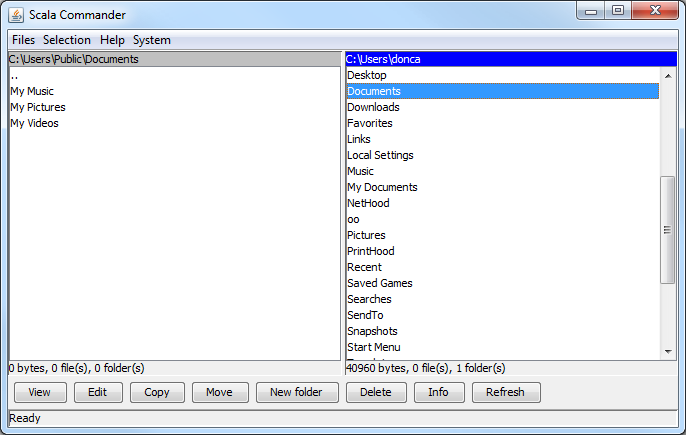
\includegraphics[width=1\textwidth]{images/scala-commander-main.png}
  \caption{Scala-Commander.}
  \label{fig:scomm_main}  
\end{figure}

The user interface is \textbf{constantly reacting to the user input}: as the user selects files and folders, a label always summarizes the selection (shows the number of selected files and folders and the total size of files). File system operations are also reactive: after clicking the \emph{Copy} button, the user can further change the selection (the files and folders to be copied) in the source panel, and can change the destination folder by navigating in the destination panel. Such changes are automatically reflected in the helper panel prompting the user at the bottom of the window. While executing a long-running operation, such as copying, the user interface is not blocked, and the user can always cancel the operation by pressing the \emph{Cancel} button.

The application is built on \emph{Scala.React} and on the the Model-View-Controller design pattern (see section \ref{sec:model-view-controller}): the model consists of \emph{event streams},  \emph{signals} and \emph{reactors}, the view listens to the model signals, and the controller interacts with the model's event streams for simple operations such as navigation, and uses \emph{reactors} for complex operations such as a file system operation.

To demonstrate the design choices, we describes two components in greater detail: the \emph{directory list} and the file system operation \emph{copy}.

\section{The directory list}

The main window consists of two directory list components: the \emph{left} list and the \emph{right} list. Both serve the same purpose: the user can see the contents of a directory, can navigate to a subdirectory or to the parent directory, and can select files and folders in the current directory. At any point of time, the directory list that the user last used is the \emph{active} list, while the other list is the \emph{inactive} list. The operations on the toolbar are always executed on the selection of the active list, and the destination of the operation (e.g. copy or move) is the directory of the inactive list.

The design of the implementation is according to the Model-View-Controller design pattern (see figure \ref{fig:mvc_pattern}). The implementation is heavily based on Scala.React concepts, resulting in significantly reduced code length and complexity, as there is no need care for event propagation, dependencies between variables, consistency, and so on.

% The directory list is a list component on the UI that displays the contents of a certain directory. The user can navigate to any subdirectory or can navigate to the parent directory. Navigation automatically updates the list. At any time, the user can select a list of files and folders and do operations on them: copy, move, delete, either by using the buttons on the toolbar or by mouse gesture (drag and drop).

\begin{figure}[h!]
\centering
\begin{tikzpicture} 
\umlemptyclass[x=0, y=-2]{DiskState}
\umlemptyclass[x=3, y=0]{DirectoryListModel}
\umlemptyclass[x=9, y=0]{DirectoryListController} 
\umlemptyclass[x=6, y=-2]{DirectoryListView} 
\umluniassoc[geometry=--]{DirectoryListModel}{DiskState} 
\umluniassoc[geometry=--]{DirectoryListController}{DirectoryListModel} 
\umluniassoc[geometry=--]{DirectoryListController}{DirectoryListView} 
\umluniassoc[geometry=--]{DirectoryListView}{DirectoryListModel} 
\umlVHdep{DirectoryListModel}{DirectoryListView}
\umlHVdep{DirectoryListView}{DirectoryListController}
\umlVHdep{DiskState}{DirectoryListModel}
\end{tikzpicture}
\caption{The directory list components.}
\label{fig:mvc_pattern}
\end{figure}


\subsection{Model}

The directory list model (class \texttt{DirectoryListModel}) holds the state of a navigable list and defines a set of operations. The operations alter the internal state of the model (e.g. change the current directory, or change selection). The model is entirely built around Scala.React concepts, such as signal variables, signal functions, event streams and reactors.

The state of the model is defined by the following signal variables:
\begin{itemize}
\item \texttt{currentDirectory: Var[Path]} --- holds the current directory (as a \texttt{java.nio.Path} object);
\item \texttt{selectedPaths: Var[Set[Path]]} --- holds the set of currently selected paths (the selection is highlighted on the user interface);
\item \texttt{active: Var[Boolean]} --- a flag representing whether the directory list is active or inactive;
\item \texttt{diskState: Var[Long]} --- a counter that is incremented whenever the disk is modified and the model need refreshing (u.i. after copying/moving/renaming/deleting, or when the user presses \emph{Refresh}).
\end{itemize}

There are also two derived signals:
\begin{itemize}

\item \texttt{currentDirContents} --- a strict signal that builds the actual list of files and folders that are located inside the current directory; it is dependent on \texttt{currentDirectory} and \texttt{diskState} (the value is just queried and ignored);

\item \texttt{selectionInfo} --- a strict signal holding an aggregated summary of what the user selected, depending \texttt{selectedPaths} and \texttt{currentDirectory}.
\end{itemize}

The model also contains three event sources, each representing an \emph{action} that is defined on the directory list:
\begin{itemize}
\item \texttt{goToParent: EventSource[Unit]} --- go to the parent of the current directory (if it exists);
\item \texttt{goToIndex: EventSource[Int]} --- go to the directory identified by the given index (index of the list \texttt{currentDirContents});
\item \texttt{selectIndices: EventSource[Set[Int]]} --- select paths identified by the given set of indexes.
\end{itemize}

Finally, the model consists of four reactors that glue together the model's state and the event sources: whenever a certain event source emits, they alter the model's state accordingly. The four reactors are the following:
\begin{itemize}
\item \texttt{goToParentReactor} --- awaits the next \texttt{goToParent} event in a loop; when it emits, sets the variable \texttt{currentDirectory} to the parent of the current directory (if it exists);
\item \texttt{goToIndexReactor} --- awaits the next index of \texttt{goToIndex} in a loop; when it emits, sets current directory to the directory identified by the index emitted by the event based on the current value of \texttt{currentDirContents};
\item \texttt{selectIndicesReactor} --- awaits the next index set of \texttt{selectIndices} in a loop; when it emits, sets the variable \texttt{selectedPaths} based on the current value of \texttt{currentDirContents};
\item \texttt{activeReactor} --- awaits the next value of the signal \texttt{active}, and if it is set to false, clears the selection (sets the variable \texttt{selectedPaths} to the empty set).
\end{itemize}

\subsection{View}

\begin{wrapfigure}{r}{0.4\textwidth}
  \centering
    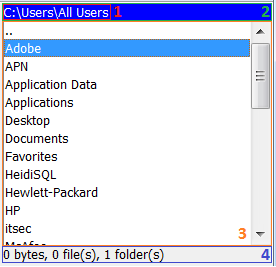
\includegraphics[width=0.35\textwidth]{images/scala-commander-directoryListView.png}
  \caption{The directory list view and its subcomponents.}
  \label{fig:scomm_main}  
\end{wrapfigure}

The directory list view (class \texttt{DirectoryListView}) is responsible for visualizing the model. It is a \texttt{scala.swing.BorderPanel}, and contains four subcomponents (figure \ref{fig:scomm_main}):
\begin{itemize}
\item \texttt{currentDirLabel}: a label displaying the full path of the current directory (marked as \texttt{1});
\item \texttt{currentDirPanel}: the panel containing the label \texttt{currentDirLabel}; the panel's background is blue for the active list and gray for the inactive list (marked as \texttt{2});
\item \texttt{listView}: a \texttt{scala.swing.ListView} component that displays the contents of the current directory, and consists of the \emph{list data} and the \emph{selection} (marked as \texttt{3});
\item \texttt{summaryLabel}: a label displaying a summary of the current selection (marked as \texttt{4}).
\end{itemize}

The view contains \texttt{observe} blocks listening to model signals, where each listener updates the appropriate Swing component. This ensures that the view is always up-to-date as the model changes.

\begin{figure}[h!]
\centering
\begin{lstlisting}[frame=single]
observe(model.currentDirectory) {
  currentDir: Path => currentDirLabel.text = currentDir.toString
}
\end{lstlisting}
\caption{The \texttt{observe} block listening to the changes of the model signal \texttt{currentDirectory}.}
\label{fig:scomm_observe_currentDir}
\end{figure}

The view listens to changes of the following model signals:
\begin{itemize}
\item \texttt{currentDirectory} --- the view updates \texttt{currentDirLabel} (see figure \ref{fig:scomm_observe_currentDir});
\item \texttt{currentDirContents} --- updates the \emph{list data} of \texttt{listView} and clears the \emph{selection};
\item \texttt{selectedPaths} --- updates the \emph{selection} of \texttt{listView};
\item \texttt{selectionInfo} --- updates \texttt{summaryLabel};
\item \texttt{active} --- updates the background of \texttt{currentDirPanel}.
\end{itemize}

\subsection{Controller}

The controller (class \texttt{DirectoryListController}) listens to the events of the view's components (extends the trait \texttt{scala.swing.Reactor}), and triggers the appropriate event sources from the model. 

The controller listens to the \emph{mouse clicks}, \emph{selection} and \emph{key} events of the \texttt{listView} component:
\begin{lstlisting}
listenTo(view.listView.mouse.clicks, view.listView.selection, view.listView.keys)
\end{lstlisting}


The controller reacts to the events generated by the above sources as follows:
\begin{lstlisting}
reactions += {
  case MouseClicked(_, _, _, 2, _) => // triggered by `mouse.clicks'
    val leadIndex = view.listView.selection.leadIndex
    model.goToIndex << leadIndex
  case ListSelectionChanged(_, _, false) => // triggered by `selection'
    if (!view.listView.updating) {
      val selection = view.listView.selection.indices.toSet
      model.selectIndices << selection
    }
  case KeyPressed(_, Key.Enter, _, _) => // triggered by `key'
    val leadIndex = view.listView.selection.leadIndex
    model.goToIndex << leadIndex
  case KeyPressed(_, Key.BackSpace, _, _) => // triggered by `key'
    model.goToParent << Unit
}
\end{lstlisting}

Note that the event handling mechanism relies heavily on Scala's pattern matching. For example, in order to listen to double click events, the first case matches events typed of the case class \texttt{MouseClicked} with the fourth parameter \texttt{clicks} fixed to the value \texttt{2}. 

\subsection{Interaction between the components}

Figure \ref{fig:scomm_event_propagation} shows the interaction between the components of a directory list when the user changes the current directory. It consists of four stages:
\begin{enumerate}
\item As the user interacts with the UI (double clicks on \texttt{listView}), the event is handled by the controller, and the controller makes event stream \texttt{goToIndex} to emit an index (the index of the line where the double clicked).
\item In the next turn, Scala.React resumes the reactor \texttt{goToIndexReactor}, which gets the index, and queries \texttt{currentDirContents} and \texttt{currentDirectory}, and updates \texttt{currentDirectory} and \texttt{selectedPaths}.
\item In the next turn, Scala.React revalidates the strict signal \texttt{currentDirContents} because its dependency \texttt{currentDirectory} was changed.
\item In the next turn, Scala.React notifies the observer blocks in the view listening to model signals   changed in previous turns; this results in the view components being updated.
\end{enumerate}

\begin{figure}[h!]
\centering
  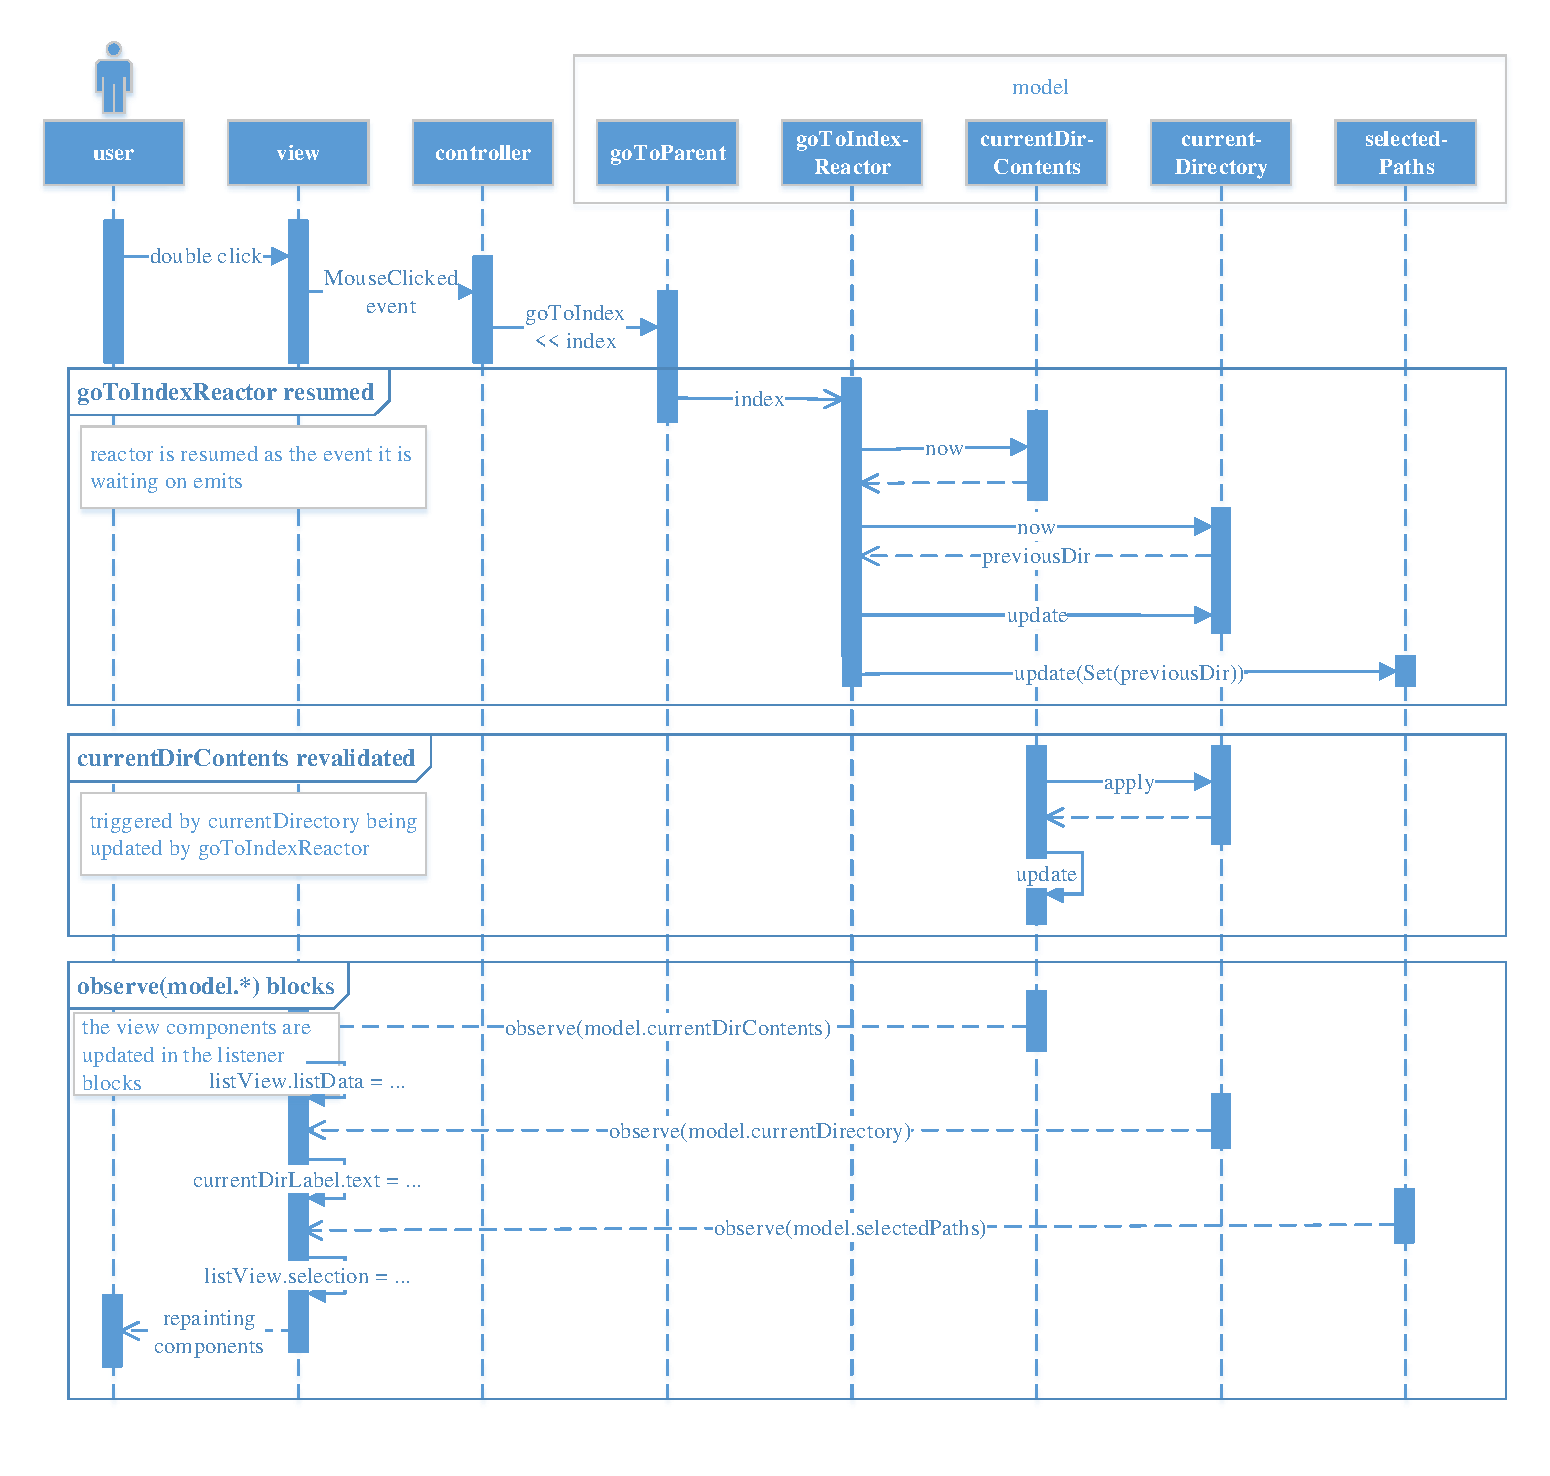
\includegraphics[width=1\textwidth]{images/scomm-event-propagation.pdf}
\caption{Sequence diagram showing the interaction between the components of a directory list when the user navigates in a directory list.}
\label{fig:scomm_event_propagation}
\end{figure}


\section{Copying files}

Copying is according to the customs of orthodox file managers: the user selects files and folders in one panel and copies them to the directory where the other panel is navigated to. Traditionally, this is implemented using modal dialogs: once the user clicks a ``Copy'' button, a modal dialog appears prompting him to confirm the action. When confirmed, another modal dialog appears showing the progress of the copying, and until the copying is over, the user cannot interact with the application. 

Our application, however, takes a slightly different approach: when clicking the ``Copy'' button, a panel at the bottom of the window appears. The panel shows the number of files and folders to be copied based on the selection in the active panel, and also contains a text box with the destination path which is the directory of the inactive panel. As the user subsequently navigates the panels, changes the selection, or switches activity, the contents of the panel are automatically updated. Once the user clicks the ``OK'' button in the panel, the selection and the destination directory is captured, and the system beings the copying: the status bar of the window shows the progress, and at any time, the user can abort the operation by pressing the ``Cancel'' button. Copying does not block the application, it remains usable. After copying is done, the directory lists are refreshed.

\subsection{Directories pane}

Because copying is defined such as to copy the selection of the \emph{active} list to the directory of the \emph{inactive} list, we need to be able to refer to the active and to the inactive directory list no matter if the left list is active and the right is inactive or vice-versa. This is where the \emph{directories pane} comes into the picture: it consists of the two directory list panels, keeps track of activity based on UI events, and the model has signal functions that always reflect certain properties of the lists. For example, the signal \texttt{activeCurrentDir} always has the value of the active directory list's path, and it is updated when either the user navigates in the active list or switches to the other list.

The model is as follows:

%\begin{figure}[h!]
%\centering

\begin{lstlisting}
class DirectoriesPaneModel(val left: DirectoryListModel,
                                    val right: DirectoryListModel) {

  val activeList = Var[DirectoryListModel]
  val inactiveList = Var[DirectoryListModel]

  val activeCurrentDir = Strict { activeList().currentDirectory() }
  val inactiveCurrentDir = Strict { inactiveList().currentDirectory() }
  val activeSelection = Strict { activeList().selectionInfo() }
  val inactiveSelection = Strict { inactiveList().selectionInfo() }
}
\end{lstlisting}

%\caption{The directories pane model.}
%\label{fig:scomm_directories_pane_model}
%\end{figure}


\subsection{Copy controller}

Copying is a single reactor: it awaits the user pressing the \emph{Copy} button on the toolbar, displays the panel, awaits the \emph{OK} button, captures the current state of the directories pane and begins copying. The user can abort the copying by pressing the \emph{Cancel} button at any time. After the copying is done or is aborted, the reactor refreshes the disk state and hides the copy panel.

A simplified version of the reactor code is as follows:

\begin{lstlisting}
Reactor.loop {
  self =>      
    self awaitNext mainWindowView.commandButtons.copyButton()
    
    displayPanel(Some(view.panel)) // display the copy panel
    self.abortOn(view.cancelButton()) { // abort on `Cancel'
      self awaitNext view.okButton() // wait until `OK'

      val sources: Set[Path] = directoriesPane.activeSelection.now.paths
      val destinationDir: Path = directoriesPane.inactiveCurrentDir
      sources.cps foreach { // do the copying
        ... self pause ... // for `abortOn' to be able to abort the copying
      }
    }
    diskState.refresh()
    displayPanel(None) // hide the copy panel
}
\end{lstlisting}


Note that the \texttt{abortOn} operator executes the body and aborts it as soon as the given reactive (the cancel button) emits. This makes it possible to cancel while waiting for the \emph{OK} button or while actually copying the files.




\chapter{FEST-Logging}\label{chap:impl_fest-logging}

Test suites testing even relatively complex applications can easily contain some hundred tests. Because UI tests, by their nature, typically take much time, the total run time of an entire test suite is usually important. In order to keep the overall runtime at minimum, it is typical to avoid the creation, initialization and the destruction of the individual UI components for each test (which might also be difficult or impossible depending on the architecture of the application). A possible option is to test entire applications and to reuse the same components between the tests.

The problem with testing entire applications throughout entire test suites is that the tests can become dependent on the internal state of the application and on the state of the UI. Thus, it is possible for one test to affect the outcome of another, e.g. one test makes a subtle change in the state of the application and makes another test fail, or, in a more extreme case, one failing test can leave the application in such a state that no other further tests will pass. Having non-independent tests can lead to fragile and unstable test systems and thus should be avoided as much as possible.

Unstable test system can very difficult to cope with. Tests can seemingly fail randomly, and it can be very difficult to reproduce failures that originate from typically a subtle change in the application's state that was made by a previous test (possibly executed many tests before). FEST supports saving screenshots anytime during a test, but the test must explicitly save it and it is usually done only on errors. Since in the case of unstable tests, the errors typically manifest themselves only in the tests that are affected by the erroneous tests' side effects, saving screenshots for failing tests does not help much on its own.

Understanding the data flow of all the tests of an entire test suite, knowing all the operations that were made on the application's state, along with screenshots made after all important steps can greatly reduce the debugging efforts of an unstable test suite and can benefit the test development and maintenance process.

\section{AspectJ-based auditing}

We introduce \emph{FEST-Logging}, an AspectJ-based solution that gathers information of the test methods and on annotated methods in the user code. The gathered information (method arguments, screenshots) are visualized in the form of a table and the entire execution tree can be inspected.

We introduce the JUnit runner \texttt{CacioFESTLoggingRunner}: enables FEST-Logging and executes the tests using the \emph{Cacio-tta} graphics stack (running the tests in the background). Running the tests with this runner is a \textbf{requirement} of FEST-Logging.

We also introduce two annotations:
\begin{itemize}
\item \texttt{GUITestBean}: a \emph{type} annotation
\item \texttt{GUITestAction}: a \emph{method} annotation.
\end{itemize}

FEST-Logging provides the following features:
\begin{itemize}
\item auditing tests --- audits the \emph{test}, \emph{setup} and \emph{teardown} methods (annotated with \texttt{@Test}, \texttt{@Before} and \texttt{@After}).
\item auditing test actions --- audits \emph{all} methods of classes annotated with \texttt{@GUITestBean};
\item screenshots of test actions --- the runtime system takes screenshots \emph{before} and \emph{after} methods annotated with \texttt{@GUITestAction} are executed;
\item screenshots of failed tests --- the runtime system takes screenshots of failing tests, failing either in their \emph{test}, \emph{setup} or \emph{teardown} methods. 
\end{itemize}

Tests using FEST-Logging generate reports as files in the folder \emph{reports/xml}. The reports can be visualized using the HTML page \emph{web/report.html}.

\subsection{Implementation}

Using a JUnit runner lets us add additional behavior to the execution of a test, similarly to advices in AspectJ. The runner \texttt{CacioFESTLoggingRunner} takes this opportunity to register the test in the object \texttt{MethodCallStack} and to execute the test. When the test is over, it captures any exceptions thrown by the test, unregisters the test from \texttt{MethodCallStack} and writes the audited data to the reports folder.

The test methods and test actions are altered by the aspect class \texttt{FESTLoggingAspect}. Here, we define a series of pointcuts, where each pointcut is to match a method annotated with a certain annotation (see figure \ref{fig:fest-logging-pointcuts}). There are also \emph{around advices} defined referring to the pointcuts, where each advice alters the execution of the method:
\begin{itemize}
\item \texttt{auditTestAndGUITestBeanMethods} --- registers and gathers the result of the advised method;
\item \texttt{takeScreenshotOfFailedTest} --- advises test methods, and takes screenshots if they throw exceptions;
\item \texttt{takeScreenshotsOfTestActions} --- takes screenshots \emph{before} and \emph{after} executing the advised method.
\end{itemize}
Each advice relies on the object \texttt{MethodCallStack}, and stores the gathered data in it.

\begin{figure}[h!]
\centering
\begin{lstlisting}
@Aspect
class FESTLoggingAspect {
  @Pointcut("execution(@org.junit.Test * *.*(..))")
  def testMethods() {}

  @Pointcut("execution(@org.junit.Before * *.*(..))")
  def beforeMethods() {}

  @Pointcut("execution(@org.junit.After * *.*(..))")
  def afterMethods() {}

  @Pointcut("execution(* (@edu.zsd.festlogging.GUITestBean *).*(..))")
  def guiTestBeanMethods() {}

  @Pointcut("execution(@edu.zsd.festlogging.GUITestAction * *.*(..))")
  def guiTestActionMethods() {}
  ...
}
\end{lstlisting}
\caption{The pointcuts matching to test methods (first three) and to test actions (last two).}
\label{fig:fest-logging-pointcuts}
\end{figure}

\subsubsection{Building the method stack}

Figure \ref{fig:fest-logging-auditMethods} shows the advice responsible for auditing. It calls the method \texttt{enterTestMethod}, proceeds the join point, and finally calls the \texttt{exitTestMethod}. This is so the class \texttt{MethodCallStack}, as the name suggests, can keep a stack of objects representing the advised methods.

\begin{figure}[h!]
\centering
\begin{lstlisting}
  @Around("testMethods() || beforeMethods() || afterMethods() || guiTestBeanMethods()")
  def auditMethods(joinPoint: ProceedingJoinPoint): AnyRef = {
    MethodCallStack.enterTestMethod(joinPoint)
    try {
      val result: AnyRef = joinPoint.proceed()
      MethodCallStack.exitTestMethod(joinPoint, result)
      result
    } catch {
      case e: Throwable =>
        MethodCallStack.exitTestMethod(joinPoint, e)
        throw e
    }
  }
\end{lstlisting}
\caption{The pointcuts matching to test methods (first three) and to test actions (last two).}
\label{fig:fest-logging-auditMethods}
\end{figure}

The class \texttt{MethodCallStack} holds a single reference named \texttt{current} of type \texttt{RunningExecution} (see figure \ref{fig:fest-logging-MethodCallStack}). This represents the \emph{top} of the stack. The very first running execution object is pushed into the stack by \texttt{CacioFESTLoggingRunner} in the form of a \texttt{RunningTestExecution} object. The class \texttt{RunningExecution} holds the advised method, the argument list, has a mutable list of child method invocations and mutable screenshot fields. 

Subsequently, when the actual test methods and the test action methods are executed, the advice \texttt{auditMethods} pushes a new \texttt{RunningTestMethodExecution} object with the parent reference set to the top of the stack. When a method terminates, the stack is ``popped'': the top object, referenced by \texttt{current}, is converted into a new \texttt{Execution} object, this \texttt{Execution} object is added to the invocation list of its parent, and this parent is then assigned to the variable \texttt{current}.

\begin{figure}[h!]
\centering
  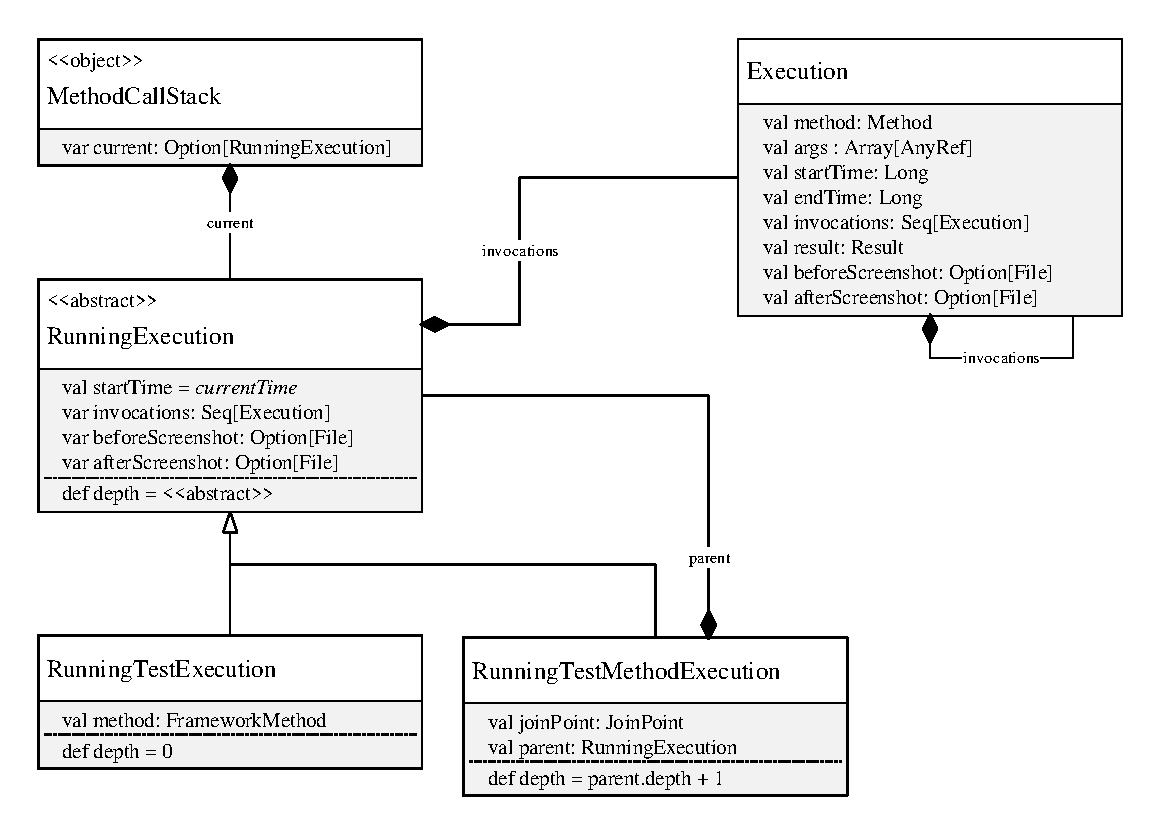
\includegraphics[width=1\textwidth]{images/FESTLogging-MethodCallStack.pdf}
\caption{Class diagram of the classes internally used by the object \texttt{MethodCallStack}. Class \texttt{RunningExecution} represents an ongoing execution (with mutable fields), and the class \texttt{Execution} represents a terminated execution (with immutable fields).}
\label{fig:fest-logging-MethodCallStack}
\end{figure}

When the execution reaches back the class \texttt{CacioFESTLoggingRunner}, the variable \texttt{current} \textbf{must be} referencing to a \texttt{RunningTestExecution} object. This also transformed to an \texttt{Execution} object, but instead of further pushing it on the stack, this object is transformed to XML format and is written to the reports folder.

\subsubsection{Taking screenshots}

There are two advices taking screenshots: \texttt{take\-Screen\-shot\-Of\-Failed\-Test} and \texttt{take\-Screen\-shots\-Of\-Test\-Actions}. Both rely on the object \texttt{MethodCallStack}: they take the topmost \texttt{Running\-Execution} object on the stack, take the screenshots into files and assign the appropriate fields in the \texttt{Running\-Execution} object. This is based on AspectJ applying multiple advices on the same method using well-defined precedence rules (which is declaration precedence in this case).

\subsection {Formatting the audited data}

Since the runtime data set can be huge for long tests runs, it is important to provide views that presents the data in an easily accessible, intuitive and adaptive form. 

A possible implementation is to generate an HTML page that contains all the data in the form of a pivot table, with a tree axis showing the call hierarchy, and the columns presenting the method arguments and other context info. The pivot table would support drill-down in the call hierarchy. This table would support the following:
\begin{itemize}
\item Closing and expanding nodes (method calls) in the call hierarchy;
\item Filtering and sorting by the context data (e.g. method names, arguments, annotations).
\end{itemize}

The following is a simple example of a test of a text editor application consisting of the following steps:
\begin{itemize}
\item create a new text file
\item enter the text ``hello'' and `` world'', respectively
\item save the text file to the disk
\item assert that the editor shows the file name in the window's title
\item assert that the file exists on the disk and has the appropriate content
\end{itemize}

Table \ref{fig:formatted_audited_data_report} shows the method calls only of the test, user action and adapter layers, along with the arguments and the return values (if applicable).

\begin{table}
\caption{Formatted audited data report}
%\rowcolors{2}{gray!25}{white}
\begin{tabular}{l l c}
%\rowcolor{gray!50}
\hline\hline

Method call & Arguments & Returns \\ [0.5ex] % inserts table heading
\hline 

\hskip 0cm EditorTest.saveNewTextFile & & PASSED \\
\hskip 3mm   EditorUserActions.createNewTextFile & & \\
\hskip 6mm     MenuAdapter.clickFileMenu & & \\ 
\hskip 6mm     MenuAdapter.clickNewTextFileMenuItem & & \\ 
\hskip 3mm   EditorUserActions.enterText & text=''hello'' & \\
\hskip 6mm     TextAreaAdapter.getCaretPosition & & 0 \\
\hskip 6mm     TextAreaAdapter.insertText & position=0, text=''hello'' & \\
\hskip 3mm   EditorUserActions.enterText & text=''world'' & \\
\hskip 6mm     TextAreaAdapter.getCaretPosition & & 5 \\
\hskip 6mm     TextAreaAdapter.insertText & position=5, text='' world'' & \\
\hskip 3mm   EditorUserActions.saveCurrentEditor & filename=''C:{\textbackslash}helloWorld.txt'' & \\
\hskip 6mm     MenuAdapter.clickFileMenu & & \\
\hskip 6mm     MenuAdapter.clickSaveMenuItem & & \\
\hskip 6mm     DialogAdapter.setFileName & filename=''C:{\textbackslash}helloWorld.txt'' & \\
\hskip 6mm     DialogAdapter.clickSaveButton & & \\
\hskip 6mm     DialogAdapter.expectToDisappear & & \\	 
\hskip 3mm   EditorUserActions.expectTitle & title=''helloWorld'' & \\
\hskip 6mm     MainWindowAdapter.expectTitle & title=''My Notepad - helloWorld'' & \\
\hskip 6mm     FileUtils.expectFileContents &
    \begin{tabular}[x]{@{}c@{}}
       path=''C:{\textbackslash}helloWorld.txt", \\
      contents=''hello world''
    \end{tabular} & \\

\hline

\end{tabular}
\label{fig:formatted_audited_data_report}
\end{table}

\section{Automatic EDT dispatch}\label{sec:edt-dispatch}

The threading model of Swing recommends that all Swing-component-related operations are to be executed on the Swing EDT thread, including those of the tests. While it is always thread-safe to use the FEST Swing fixtures, there are some cases when the methods exposed in a fixture are not enough and one needs to access the underlying component. Direct interaction with Swing components with the purpose of testing must be delegated to the EDT thread (unless the tests can become unstable). Fortunately, FEST-Swing offers the class \texttt{GuiActionRunner} that provides a simple way to execute tasks or queries on the EDT, such as:
\begin{lstlisting}
def requireCurrentDirBackground(color: Color) = {
  GuiActionRunner.execute(new GuiTask {
    override def executeInEDT(): Unit = {
      assertEquals(color, currentDirPanel.component().getBackground)
    }
  })
}
\end{lstlisting}
It is even possible to do assertion in a \texttt{GuiTask} because if the assertion fails, the \texttt{Assertion\-Error} exception is propagated back the test thread with a merged stack trace that helps debugging. However, this is still much boilerplate code to write just for a simple assertion.

To offer a solution to this problem, we present the annotation \texttt{ExecuteInEDT} as part of \emph{FEST-Logging} library. When an annotated method is called on the test thread, the method is seamlessly and transparently delegated to the Swing EDT thread, and the test thread awaits the result (the return value or the exception). This leads to less effort from the developer's side, and at the same time, increases security on the tests' correctness. The above example is equivalent to the following:
\begin{lstlisting}
@ExecuteInEDT
def requireCurrentDirBackground(color: Color): Unit = {
  assertEquals(color, currentDirPanel.component().getBackground)
}
\end{lstlisting}

\subsection{Implementation}\label{sec:edt-dispatch}

We define a pointcut that matches methods annotated with \texttt{ExecuteInEDT}, and we use an \emph{around advice} to delegate the invocation to Swing EDT:
\begin{lstlisting}
@Pointcut("execution(@edu.zsd.festlogging.ExecuteInEDT * *.*(..))")
def executeInEDTMethods() {}

@Around("executeInEDTMethods()")
def executeInEDT(joinPoint: ProceedingJoinPoint) : AnyRef = {
  GuiActionRunner.execute(new GuiQuery[AnyRef] {
    override def executeInEDT(): AnyRef = joinPoint.proceed()
  })
}
\end{lstlisting}

The method \texttt{GuiActionRunner.execute} takes a single \texttt{query} argument and executes it on Swing EDT. If the current thread is already Swing EDT, the method directly executes the argument and returns the value, otherwise it uses \texttt{SwingUtilities.invokeLater} to execute the method and wait for the response. In case the method threw an exception, the stack trace is \textbf{merged} with the invocation stack of the \texttt{GuiActionRunner.execute} method, resulting in an exception that looks just as if the query was executed synchronously on the test thread.


\section{Case study: Scala Commander}

We are using FEST-Logging for the UI-tests of Scala Commander. 







\appendix

\chapter{Scala CPS plugin examples}\label{chap:cps-examples}

\begin{figure}[h!]
\begin{lstlisting}
val v1 = reset {
  shift { k: (Int=>Int) =>
    k(7)
  } + 1
} * 2
println(v1) // prints 16
\end{lstlisting}
\caption{A simple numeric example. The value of the \texttt{reset} block is equal to the value of the \texttt{shift} block plus one. The \texttt{shift}, block gets the rest of the continuation in the form of the function \texttt{k}, which in this case is the function \(x + 1\). The shift block invokes \texttt{k} with the argument 7 and returns the resulting value 8, which is then the value of the \texttt{reset} block. This value is then multiplied by 2 (outside the continuation), so the printed value is 16.}
\label{fig:example_cps_1}
\end{figure}




\begin{figure}[h!]
\begin{lstlisting}
val v2 = reset {
  shift { k: (Int=>Int) =>
    k(k(k(7)))
  } + 1
} * 2
println(v2) // prints 20
\end{lstlisting}
\caption{Example showing that the rest of the continuation may be called multiple times. In this case, the rest of the continuation is invoked three times. The final result of the continuation is multiplied by 2 outside the continuation (resulting in the value 20).}
\label{fig:example_cps_2}
\end{figure}




\begin{figure}[h!] 
\begin{lstlisting}
val result = reset {
  println("entering first shift")
  val firstShift = shift { k: (Int => Int) =>
      val res = k(0)
      println(s"exiting first shift, res = $res")
      res
  } + 1

  println(s"firstShift = $firstShift; entering second shift")
  val secondShift = shift { k: (Int => Int) =>
      val res: Int = k(firstShift)
      println(s"exiting second shift, res = $res")
      res
  } + 1
  println(s"secondShift = $secondShift; returning the reset")

  secondShift
}

println(s"result = $result")

// entering first shift
// firstShift = 1; entering second shift
// secondShift = 2; returning the reset
// exiting second shift, res = 2
// exiting first shift, res = 2
// result = 2
\end{lstlisting}
\caption{Example showing the control flow throughout the reset block when there is more than one shift block. Notice the similarity with multiple function calls.}
\label{fig:example_cps_step_by_step}
\end{figure}



\begin{figure}[h!] 
\begin{lstlisting}
import scala.util.continuations._

object TwelveDaysOfChristmas extends App {
  val daysAndGifts = Seq(
    ("First", "a Patridge in a Pear Tree"),
    ("Second", "Two Turtle Doves"),
    ("Third", "Three French Hens")
  )
  val days = daysAndGifts.map(_._1)
  val gifts = daysAndGifts.map(_._2)

  val carol: List[String] = reset {
    val dayIndex: Int = shift {
      verse: (Int => List[String]) =>
        (0 to days.length - 1).foldRight(List.empty[String])((day, list) => "" :: verse(day) ::: list)
    }

    // the continuation below this line calculated a single verse for the day identified by `dayIndex`
    val dayLine = s"On the ${days(dayIndex)} day of Christmas my true love sent to me"
    val giftIndex: Int = shift {
      line: (Int => String) =>
        dayLine :: (0 to dayIndex).foldLeft(List.empty[String])((list, gift) => line(gift) :: list)
    }

    // the continuation below this line calculates a single line of a verse, the line identified by `giftIndex`

    val gift = gifts(giftIndex)
    val line = if (dayIndex == 0) {
      s"$gift."
    } else if (giftIndex > 0) {
      s"$gift,"
    } else {
      s"and $gift."
    }
    line
  }
  carol.foreach(println(_))

  /*
  On the First day of Christmas my true love sent to me
  a Patridge in a Pear Tree.

  On the Second day of Christmas my true love sent to me
  Two Turtle Doves,
  and a Patridge in a Pear Tree.

  On the Third day of Christmas my true love sent to me
  Three French Hens,
  Two Turtle Doves,
  and a Patridge in a Pear Tree.  */
}
\end{lstlisting}
\caption{An example printing the first three verses of the well-known Christmas carol ``The Twelve Days of Christmas''. Notice the answer type modification.}
\label{fig:example_twelve_days}
\end{figure}






\begin{figure}

    \begin{minipage}{.7\linewidth}
      \centering
        \begin{lstlisting}
import scala.util.continuations._
import scala.swing._

object ContinuationsSwingApp extends SimpleSwingApplication {

  var continue: (Unit => Unit) = { _ => run()}

  def run() {
    reset {
      val first = ask("What is your first name?")
      val last = ask("What is your last name?")
      label.text = s"Hello, $first $last!"
    }
  }

  def ask(prompt: String): String@cpsParam[Unit, Unit] = {
    label.text = prompt
    shift {
      k: (Unit => Unit) => {
        continue = k
      }
    }
    textField.text
  }

  val textField = new TextArea(10, 40)
  val label = new Label("Welcome to the demo app")
  val button = new Button(new Action("Next") {
    override def apply(): Unit = continue()
  })

  override def top: swing.Frame = new MainFrame {
    contents = new BorderPanel {
      add(label, BorderPanel.Position.North)
      add(textField, BorderPanel.Position.Center)
      add(button, BorderPanel.Position.South)
    }
  }
}
\end{lstlisting}
    \end{minipage}%
    \begin{minipage}{.3\linewidth}
      \centering

        \begin{tabular}{c}
Step1:\\
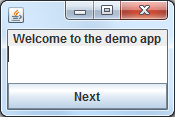
\includegraphics[width=0.9\linewidth]{images/swing-demo-step1.png} \\[0.7cm] 
Step2:\\
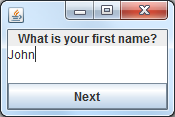
\includegraphics[width=0.9\linewidth]{images/swing-demo-step2.png} \\[0.7cm]
Step3:\\
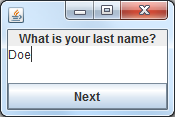
\includegraphics[width=0.9\linewidth]{images/swing-demo-step3.png} \\[0.7cm]
Step4:\\
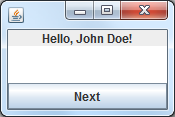
\includegraphics[width=0.9\linewidth]{images/swing-demo-step4.png} \\
\end{tabular}

    \end{minipage} 


\caption{A simple Swing application with an event-based control flow defined in imperative style (see method \texttt{run}). For each question, the flow is suspended and the \texttt{shift} blocks assigns the rest of the continuation to a variable. Pushing the button resumes the continuation.}
\label{fig:example_twelve_days}
\end{figure}





\chapter{Scala.React examples}\label{chap:scala-react-examples}


\begin{figure}[h!] 
\begin{lstlisting}
object MyDomain extends Domain {
  val scheduler = new SwingScheduler()
  val engine = new Engine
} import MyDomain._

object ScalaReactLineDrawing extends SimpleSwingApplication with Observing{
  override def main(args: Array[String]) {
    schedule { startup(args) }
    start() // starts the scala-react engine
  }
  override def top: Frame = new MainFrame() {
    contents = new FlowPanel() {
      val mouseDown = EventSource[Point]
      val mouseMove = EventSource[Point]
      val mouseUp = EventSource[Point]

      val mainProgramFlow = Reactor.loop {
        self =>
        // step 1
          val path = new Path(self await mouseDown)
          self.loopUntil(mouseUp) {
            // step 2
            val m = self awaitNext mouseMove
            path.lineTo(m)
            draw(path)
          }
          path.close() // step 3
          draw(path)
      }

      listenTo(mouse.clicks, mouse.moves) // scala.swing events
      reactions += {
        case MousePressed(_, point, _, _, _) => mouseDown << point
        case MouseReleased(_, point, _, _, _) => mouseUp << point
        case MouseDragged(_, point, _) => mouseMove << point
      }
      class Path(var positions: Seq[Point]) {
        def this(pos: Point) = this(Seq(pos))
        def lineTo(pos: Point) { positions = positions :+ pos }
        def close() { positions = positions :+ positions.head }
      }
      var pathDrawn = new Path(new Point(0, 0))
      def draw(path: Path) { pathDrawn = path; repaint() }
      override protected def paintComponent(g: swing.Graphics2D): Unit = {
        super.paintComponent(g)
        val xPoints = pathDrawn.positions.map(pos => pos.x).toArray
        val yPoints = pathDrawn.positions.map(pos => pos.y).toArray
        g.setColor(Color.BLACK)
        g.drawPolyline(xPoints, yPoints, pathDrawn.positions.length)
} } } }
\end{lstlisting}
\caption{A sample application painting a closed line with the mouse using Scala.React \emph{reactor} and \emph{event streams}.}
\label{fig:example_scala-react-line-drawing}
\end{figure}

















	
{ \renewcommand{\baselinestretch}{0.8}\normalsize %
  \setlength{\itemsep}{-2.4mm}
  \setlength{\bibspacing}{0.67\baselineskip}

  \bibliographystyle{abbrvnat}
  % \bibliographystyle{plain}
  % \bibliographystyle{unsrt}
  \bibliography{paper_bibliography}
}


\end{document}
